\documentclass{report}%
\usepackage[T1]{fontenc}%
\usepackage[utf8]{inputenc}%
\usepackage{lmodern}%
\usepackage{textcomp}%
\usepackage{lastpage}%
\usepackage{geometry}%
\geometry{bindingoffset=0.2in,left=1in,right=1in,top=1in,bottom=1in,footskip=0.25in}%
\usepackage{amsmath}%
\usepackage{hyperref}%
\usepackage{graphicx}%
\usepackage{longtable}%
\usepackage{tabu}%
\usepackage[table]{xcolor}%
\usepackage{fancyhdr}%
%
\linespread{1.5}%
\title{\textbf{Arline: Benchmarks} \\
                    Automated benchmarking platform for quantum compilers, quantum hardware and quantum algorithms \\
                    \vspace{2cm}
                    \normalsize{\textbf{Automatically generated report}} \\
                    \vspace{0.5cm}
                    \normalsize{\textbf{by Arline Benchmarks}}
                    \vspace{2cm}
                    }%
\author{https://github.com/ArlineQ/arline\_benchmarks}%
\date{\today}%
\fancypagestyle{header}{%
\renewcommand{\headrulewidth}{0pt}%
\renewcommand{\footrulewidth}{0pt}%
\fancyhead{%
}%
\fancyfoot{%
}%
\fancyhead[R]{%
\leftmark%
}%
\fancyfoot[R]{%
Page \thepage\ of \pageref{LastPage}%
}%
\fancyfoot[L]{%
\footnotesize{\textbf{Automatically generated report by Arline Benchmarks \\
                    https://github.com/ArlineQ/arline\_benchmarks}}%
}%
}%
%
\begin{document}%
\normalsize%
\maketitle%
\tableofcontents%
\pagestyle{header}%
\chapter{Overview}%
\label{chap:Overview}%
Quantum compilation is a problem of translating quantum algorithm to the set of low-level
                    hardware instructions to be executed on the quantum processor. Efficient compilation and circuit
                    optimisation (finding an optimal sequence of gates for the desired quantum computation) is immense
                    importance for practical applications and is necessary for further progress towards scalable quantum
                    computation.\bigskip

                    \noindent{The importance of optimal quantum compilation stems from the fact that noisy
                    intermediate-scale quantum (NISQ) devices suffer from unavoidable noise caused by individual gates.
                    Extreme susceptibility of quantum computation to noise is the crucial problem that hinders
                    the development of large-scale quantum computers. By the means of optimising gate count in the
                    quantum circuit, it is possible to significantly reduce hardware errors.} \bigskip

                    \noindent{Optimal (or near-optimal) circuit compilation is an extremely challenging task due to
                    additional constraints imposed by hardware configuration, such as restricted qubit connectivity
                    and hardware-native gate set. Finding optimal gate sequences for a given quantum circuit with all
                    imposed constraints is an open problem. For two-qubit circuits, the KAK algorithm is an example
                    of the efficient compilation algorithm, that is used in practical applications.} \bigskip

                    \noindent{The subroutines for quantum circuit optimisation, mapping and routing for particular
                    hardware connectivity are an integral part of existing quantum software frameworks. The complexity
                    and diversity of various quantum compilation algorithms create a necessity of cross-benchmarking and
                    comparison between different compiler frameworks. It worth to note, that the problem of hardware
                    benchmarking often arises in classical computing, where hardware is compared based on their
                    performance on a set of predefined tests.} \\ \\ \bigskip

                    \noindent{Arline Benchmarks}\footnotemark%
\footnotetext{\textbf{Disclaimer.} This report was prepared using open source program Arline
                    Benchmarks and is provided "AS IS", "AS AVAILABLE", and all warranties, express or implied,
                    are disclaimed.\bigskip

                    Neither the authors of the Arline Benchmarks program, nor any of their employees, nor any of
                    their contractors, subcontractors or their employees, makes any warranty, express or implied, or
                    assumes any legal liability or responsibility for the accuracy, completeness, or any third party's
                    use or the results of such use of any information, apparatus, product, or process disclosed,
                    or represents that its use would not infringe privately owned rights.\bigskip

                    Readers are cautioned that information contained in this report is only current as of the
                    respective dates of such information. The technical condition, analyzed program code,
                    comparative results may have changed since those dates. Readers are advised to review only the most
                    recent document for the most current information. \\ \bigskip}
                    %
platform is created to solve benchmarking problem in the quantum world and aims to provide a
                    fair comparison between compilers for various quantum hardware and quantum algorithms.
                    %
\section{Frameworks }%
\label{sec:Frameworks}%
Below we list compilation frameworks used in the benchmarking run:%
\begin{itemize}%
\item%
\textbf{IBM Qiskit}\footnotemark%
\footnotetext{IBM and Qiskit are trademarks of International
                            Business Machines Corporation, registered in many jurisdictions worldwide.}%
v0.34.2 (open-source).\textbf{Qiskit} is an open-source framework for working with quantum computers at the
                            level of circuits, pulses, and algorithms. Qiskit transpiler combines mapping and
                            compression subroutines. The transpiler has three levels of optimization, in our report,
                            we invoke the most advanced optimization level (3).%
\begin{itemize}%
\item%
Compression/optimization algorithm relies on \textbf{commutative cancellations of
                                gates, aggregation of single-qubit gates, removal of diagonal gates before
                                measurement.}%
\item%
Routing and mapping algorithms are based on construction of a
                                \textbf{basic, stochastic or lookahead swap network.}%
\item%
The output circuit gate set: %
$U_1$, $U_2$, $U_3$, $CNOT$, $I$.%
\end{itemize}%
\end{itemize}%
\begin{itemize}%
\item%
\textbf{Google Cirq library} %
v0.13.1 (open-source). \textbf{Cirq} has been developed by Google AI Quantum Team. Cirq supports
                            mapping/routing operations and tailored towards specific grid-like qubit coupling
                            topologies.%
\begin{itemize}%
\item%
The compression subroutines include \textbf{pushing Pauli gates and phased
                                Pauli gates to the end of the circuit, merging single-qubit gates and dropping
                                negligible gates and empty moments}.%
\item%
Routing and mapping methods are based on a \textbf{greedy swap insertion
                                strategy.}%
\item%
The output circuit gate set: $R_x$, $R_z$, $CZ$.%
\end{itemize}%
\end{itemize}

%
\section{Definitions}%
\label{sec:Definitions}%
We define compression factor ($CF$) for a particular class of gates ($G$)
                    (e.g. single-qubit gates, two-qubit gates) averaged over circuits ($C$) as:%
\begin{itemize}%
\item%
Compression factor greater then unity ($CF(G)>1$) corresponds to a successful compression
                        (the gate count of the gate ($G$) in the output circuit is less compared to the input circuit).
                        Similarly, compression factor less then unity ($CF(G)<1$) corresponds to
                        unsuccessful compression (the output circuit contains more gates of type ($G$)
                        compared to the input circuit).%
\begin{alignat*}{2}%
CF(G) =\left \langle  \frac{\textrm{gate count}
                        (G, C_i)_{\textrm{before}}}{\textrm{gate count}(G, C_i)_{\textrm{after}}} \right\rangle_{C}.%
\end{alignat*}%
\item%
Circuits \textbf{before} and \textbf{after} correspond to initial and
                        final compilation stages. In the present report, we usually assume that the initial stage is
                        target generation, the final stage is typically either \textbf{compression} or
                        \textbf{rebase} to the output hardware gate set.
                        %
\end{itemize}%
As an additional metric that defines a circuit cost we use the following
                    circuit cost function:%
\begin{alignat*}{2}%
C = -\log{\left(K^d \prod_i F^{1q}_i \prod_j F^{2q}_j\right)},%
\end{alignat*}%
where $C$ - circuit cost, $K$ - factor that penalises deep circuits,
                    $d$ - circuit depth, $F^{1q}_i$ - fidelity of single qubit gates,
                    $F^{2q}_j$ - fidelity of two qubit gates. 

%
\section{Metrics}%
\label{sec:Metrics}%
\begin{itemize}%
\item%
Depth%
\item%
Total Gate Count%
\item%
Single-Qubit Gate Count%
\item%
Two-Qubit Gate Count%
\item%
Single-Qubit Gate Depth%
\item%
Two-Qubit Gate Depth%
\item%
Circuit Cost Function%
\item%
Execution Time%
\end{itemize}%
Note that in most cases single-qubit gate count and single-qubit gate compression factor
                    have only limited meaning as a metric of compiler performance. This is because single-qubit
                    gate count is very sensitive to the choice single-qubit basisgates (e.g. $U_3$ is equivalent
                    to a combination of 3 rotation gates $R_x$, $R_y$ and $R_z$).

%
\section{Hardware Backends }%
\label{sec:HardwareBackends}%
Hardware backends are defined in open-source \textbf{Arline Quantum} library %
\linebreak%
\hyperref[]{https://github.com/ArlineQ/arline\_quantum}%
. Names of hardware backends reflect gate set and connectivity. E.g. IbmAll2All16Q
                    corresponds to a 16-qubit fully-connected mock backend with the native gate set of the IBM
                    quantum hardware. \bigskip%


\begin{figure}[h!]%
\centering%
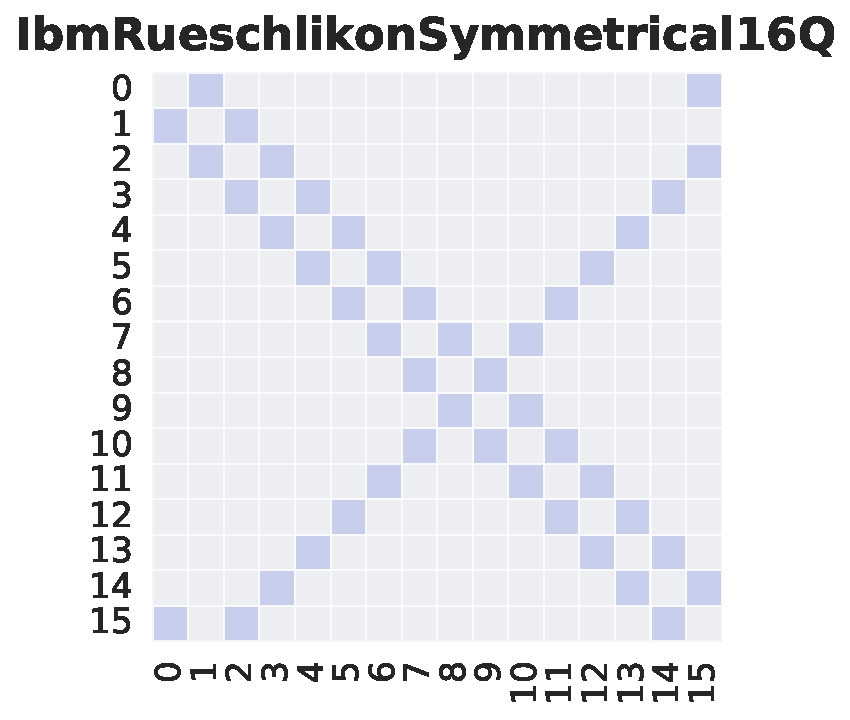
\includegraphics[width=0.3\textwidth]{/home/nathanschnitzer/arline_benchmarks/configs/compression/results/figures/coupling_map_ibmrueschlikonsymmetrical16q.pdf}%
\caption{IbmRueschlikonSymmetrical16Q hardware coupling map: adjacency matrix.}%
\end{figure}

%


\begin{figure}[h!]%
\centering%
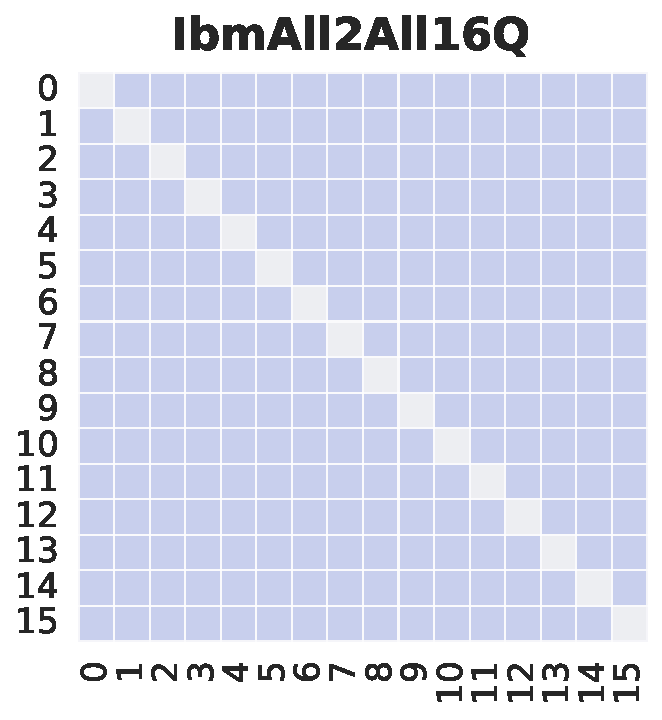
\includegraphics[width=0.3\textwidth]{/home/nathanschnitzer/arline_benchmarks/configs/compression/results/figures/coupling_map_ibmall2all16q.pdf}%
\caption{IbmAll2All16Q hardware coupling map: adjacency matrix.}%
\end{figure}

%
\clearpage

%
\section{Compilation Pipelines}%
\label{sec:CompilationPipelines}%

%
\textbf{Compilation pipeline} is a sequence of compilation routines,
                which typically consist of three main stages:%
\begin{enumerate}%
\item%
\textbf{Unroll} (optional) for the three-qubit gates;%
\item%
\textbf{Mapping} and \textbf{routing} of the original circuit to
                    a hardware topology, further \textbf{mapping};%
\item%
\textbf{Compression} of the circuit that reduces the number of gates involved;%
\item%
\textbf{Rebase} (optional) of the final gate sequence into a particular gate set;%
\end{enumerate}%
Summary of compilation pipelines settings used in the current report is presented below. \\ %
Number of pipelines for benchmarking: \textbf{2}%
\begin{itemize}%
\item%
Pipeline name: \textbf{QiskitPl}%
\begin{enumerate}%
\item%
Stage name: \textbf{mapping\_compression}%
\end{enumerate}%
\item%
Pipeline name: \textbf{CirqPl}%
\begin{enumerate}%
\item%
Stage name: \textbf{mapping\_compression}%
\end{enumerate}%
\end{itemize}%
\section{System Info}%
\label{sec:SystemInfo}%
\begin{itemize}%
\item%
Platform: Linux{-}5.13.0{-}1029{-}azure{-}x86\_64{-}with{-}glibc2.29%
\item%
Processor: AMD EPYC 7763 64{-}Core Processor%
\item%
Memory: 15.6 Gb%
\end{itemize}

%
\section{Targets}%
\label{sec:Targets}%
Target is a quantum circuit subject to compilation. List of target generators: %
\begin{itemize}%
\item%
Target generator type: random circuits from [Clifford + T] gate set:%
\begin{itemize}%
\item%
Number of circuits: 10%
\item%
Gates frequencies: {[}Cnot: 0.152, H: 0.17, S: 0.161, Sd: 0.168, T: 0.172, Td: 0.177{]}%
\item%
Mean number of qubits: 2.0%
\item%
Mean circuit depth per circuit: 84.7%
\item%
Mean single{-}qubit gate count per circuit: 101.7%
\item%
Mean two{-}qubit gate count per circuit: 18.3%
\item%
Mean total gate count per circuit: 120.0%
\end{itemize}%
\end{itemize}%
\begin{itemize}%
\item%
Target generator type: random circuits from [CNOT, U$_3$] gate set:%
\begin{itemize}%
\item%
Number of circuits: 10%
\item%
Gates frequencies: {[}Cnot: 0.515, U3: 0.485{]}%
\item%
Mean number of qubits: 2.0%
\item%
Mean circuit depth per circuit: 108.0%
\item%
Mean single{-}qubit gate count per circuit: 58.2%
\item%
Mean two{-}qubit gate count per circuit: 61.8%
\item%
Mean total gate count per circuit: 120.0%
\end{itemize}%
\end{itemize}%
\begin{itemize}%
\item%
Target generator type: random circuits from [Clifford + T] gate set:%
\begin{itemize}%
\item%
Number of circuits: 10%
\item%
Gates frequencies: {[}Cnot: 0.743, H: 0.061, S: 0.045, Sd: 0.049, T: 0.054, Td: 0.048{]}%
\item%
Mean number of qubits: 16.0%
\item%
Mean circuit depth per circuit: 33.8%
\item%
Mean single{-}qubit gate count per circuit: 30.9%
\item%
Mean two{-}qubit gate count per circuit: 89.1%
\item%
Mean total gate count per circuit: 120.0%
\end{itemize}%
\end{itemize}%
\begin{itemize}%
\item%
Target generator type: random circuits from [CNOT, U$_3$] gate set:%
\begin{itemize}%
\item%
Number of circuits: 10%
\item%
Gates frequencies: {[}Cnot: 0.926, U3: 0.074{]}%
\item%
Mean number of qubits: 16.0%
\item%
Mean circuit depth per circuit: 36.9%
\item%
Mean single{-}qubit gate count per circuit: 8.9%
\item%
Mean two{-}qubit gate count per circuit: 111.1%
\item%
Mean total gate count per circuit: 120.0%
\end{itemize}%
\end{itemize}%
\begin{itemize}%
\item%
Target generator type: QASM circuits for arithmetic blocks:%
\begin{itemize}%
\item%
Number of circuits: 5%
\item%
Gates frequencies: {[}Cnot: 0.445, H: 0.123, T: 0.246, Td: 0.185, X: 0.001{]}%
\item%
Mean number of qubits: 16.0%
\item%
Mean circuit depth per circuit: 165.2%
\item%
Mean single{-}qubit gate count per circuit: 184.7%
\item%
Mean two{-}qubit gate count per circuit: 148.2%
\item%
Mean total gate count per circuit: 332.8%
\end{itemize}%
\end{itemize}

%
\chapter{Comparison with KAK Decomposition: Two-Qubit Circuits}%
\label{chap:ComparisonwithKAKDecompositionTwo{-}QubitCircuits}%
\section{Cartan decomposition}%
\label{sec:Cartandecomposition}%
Cartan decomposition (KAK decomposition) provides theoretical
                        $CNOT$-optimal schemes for two-qubit circuits (Figure \ref{fig:KAK}).\bigskip%


\begin{figure}[h]%
\centering%
\includegraphics[width=0.7\textwidth]{/home/nathanschnitzer/.local/lib/python3.8/site-packages/arline_benchmarks/reports/./kak_scheme.png}%
\caption{\label{fig:KAK}KAK decomposition scheme for two-qubit circuits.}%
\end{figure}

%
\noindent{Arbitrary two-qubit unitary can be represented using $U_3$ and $CNOT$ gates
                        with no more than: }%
\renewcommand{\arraystretch}{1.5}%
\begin{longtabu}{|l|l|l|}%
\hline%
\rowcolor{lightgray}%
\textbf{Metrics}&\textbf{Gate Count}&\textbf{Depth}\\%
\hline%
\endhead%
\multicolumn{3}{|r|}{Continued on Next Page}\\%
\hline%
\endfoot%
\endlastfoot%
$CNOT$&3&3\\%
\hline%
$U_3$&8&4\\%
\hline%
Total&11&7\\%
\hline%
\end{longtabu}

%
\newpage%
\chapter{Target: Random Circuits from [Clifford + T] Gate Set}%
\label{chap:TargetRandomCircuitsfromClifford+TGateSet}%
\section{Hardware: IbmAll2All2Q}%
\label{sec:HardwareIbmAll2All2Q}%

%
\subsection*{Metrics for each stage of compilation pipeline and aggregate compression factor
                    (initial/final)}%
\label{subsec:Metricsforeachstageofcompilationpipelineandaggregatecompressionfactor(initial/final)}%

%
Note that in most cases single-qubit gate count and single-qubit gate compression factor
                have only limited meaning as a metric of compiler performance.This is because single-qubit
                gate count is very sensitive to the choice single-qubit basis gates (e.g. $U_3$ is
                equivalent to a combination of 3 rotation gates $R_x$, $R_y$ and $R_z$).%


\begin{figure}[h!]%
\centering%
\includegraphics[width=0.4\textwidth]{/home/nathanschnitzer/arline_benchmarks/configs/compression/results/figures/kak/random_chain_clifford_t_2q_120/IbmAll2All2Q/bars_depth.pdf}%
\centering%
\includegraphics[width=0.4\textwidth]{/home/nathanschnitzer/arline_benchmarks/configs/compression/results/figures/kak/random_chain_clifford_t_2q_120/IbmAll2All2Q/bars_total_gate_count.pdf}%
\linebreak%
\centering%
\includegraphics[width=0.4\textwidth]{/home/nathanschnitzer/arline_benchmarks/configs/compression/results/figures/kak/random_chain_clifford_t_2q_120/IbmAll2All2Q/bars_single_qubit_gate_count.pdf}%
\centering%
\includegraphics[width=0.4\textwidth]{/home/nathanschnitzer/arline_benchmarks/configs/compression/results/figures/kak/random_chain_clifford_t_2q_120/IbmAll2All2Q/bars_two_qubit_gate_count.pdf}%
\linebreak%
\centering%
\includegraphics[width=0.4\textwidth]{/home/nathanschnitzer/arline_benchmarks/configs/compression/results/figures/kak/random_chain_clifford_t_2q_120/IbmAll2All2Q/bars_single_qubit_gate_depth.pdf}%
\centering%
\includegraphics[width=0.4\textwidth]{/home/nathanschnitzer/arline_benchmarks/configs/compression/results/figures/kak/random_chain_clifford_t_2q_120/IbmAll2All2Q/bars_two_qubit_gate_depth.pdf}%
\linebreak%
\caption{Circuits metrics for each compilation pipeline stage for IbmAll2All2Q.}%
\end{figure}

%


\begin{figure}[h!]%
\centering%
\includegraphics[width=0.4\textwidth]{/home/nathanschnitzer/arline_benchmarks/configs/compression/results/figures/kak/random_chain_clifford_t_2q_120/IbmAll2All2Q/bars_circuit_cost_function.pdf}%
\caption{Circuit cost function for IbmAll2All2Q.}%
\end{figure}

%


\begin{figure}[h!]%
\centering%
\includegraphics[width=0.4\textwidth]{/home/nathanschnitzer/arline_benchmarks/configs/compression/results/figures/kak/random_chain_clifford_t_2q_120/IbmAll2All2Q/compression_target_analysis_to_mapping_compression.pdf}%
\centering%
\includegraphics[width=0.4\textwidth]{/home/nathanschnitzer/arline_benchmarks/configs/compression/results/figures/kak/random_chain_clifford_t_2q_120/IbmAll2All2Q/comp_radar_target_analysis_to_mapping_compression.pdf}%
\caption{Compression factor ($CF$) between target and final compilation stage for IbmAll2All2Q
                        (histogram and radar plot).
                        }%
\end{figure}

%
\clearpage%
\subsection*{Gate composition for each compilation pipeline stage}%
\label{subsec:Gatecompositionforeachcompilationpipelinestage}%

%


\begin{figure}[h!]%
\centering%
\includegraphics[width=0.4\textwidth]{/home/nathanschnitzer/arline_benchmarks/configs/compression/results/figures/kak/random_chain_clifford_t_2q_120/IbmAll2All2Q/gate_composition_heatmap_qiskitpl.pdf}%
\centering%
\includegraphics[width=0.4\textwidth]{/home/nathanschnitzer/arline_benchmarks/configs/compression/results/figures/kak/random_chain_clifford_t_2q_120/IbmAll2All2Q/gate_composition_heatmap_cirqpl.pdf}%
\linebreak%
\caption{Gate frequencies in each pipeline stage for IbmAll2All2Q.}%
\end{figure}

%
\subsection*{Execution time stats }%
\label{subsec:Executiontimestats}%

%
Here we present stats about execution time (in seconds)
                spent by frameworks for each compilation stage.%


\begin{figure}[h!]%
\centering%
\includegraphics[width=0.4\textwidth]{/home/nathanschnitzer/arline_benchmarks/configs/compression/results/figures/kak/random_chain_clifford_t_2q_120/IbmAll2All2Q/bars_execution_time.pdf}%
\caption{Mean execution time of each compilation stage for IbmAll2All2Q.}%
\end{figure}

%
\subsection*{Summary stats (averaged over target circuits) by pipeline}%
\label{subsec:Summarystats(averagedovertargetcircuits)bypipeline}%

%
\renewcommand{\arraystretch}{1.5}%
\begin{longtabu}{|l|l|l|}%
\hline%
\rowcolor{lightgray}%
\textbf{Metrics}&\textbf{Min}&\textbf{Max}\\%
\hline%
\endhead%
\multicolumn{3}{|r|}{Continued on Next Page}\\%
\hline%
\endfoot%
\endlastfoot%
Depth&QiskitPl&CirqPl\\%
\hline%
Total Gate Count&QiskitPl&CirqPl\\%
\hline%
Single{-}Qubit Gate Count&QiskitPl&CirqPl\\%
\hline%
Two{-}Qubit Gate Count&CirqPl&CirqPl\\%
\hline%
Single{-}Qubit Gate Depth&QiskitPl&CirqPl\\%
\hline%
Two{-}Qubit Gate Depth&CirqPl&CirqPl\\%
\hline%
Circuit Cost Function&QiskitPl&CirqPl\\%
\hline%
Execution Time&CirqPl&QiskitPl\\%
\hline%
\end{longtabu}%
\subsection*{Cluster analytics }%
\label{subsec:Clusteranalytics}%

%
Scatter plots with axes representing: depth, (input/output) single-qubit gate count,
                (input/output) two-qubit gate count, (input/output) total gate count and execution time.%


\begin{figure}[h!]%
\centering%
\includegraphics[width=0.4\textwidth]{/home/nathanschnitzer/arline_benchmarks/configs/compression/results/figures/kak/random_chain_clifford_t_2q_120/IbmAll2All2Q/scatter_total_gate_count_vs_depth.pdf}%
\centering%
\includegraphics[width=0.4\textwidth]{/home/nathanschnitzer/arline_benchmarks/configs/compression/results/figures/kak/random_chain_clifford_t_2q_120/IbmAll2All2Q/scatter_two_qubit_gate_count_vs_depth.pdf}%
\linebreak%
\centering%
\includegraphics[width=0.4\textwidth]{/home/nathanschnitzer/arline_benchmarks/configs/compression/results/figures/kak/random_chain_clifford_t_2q_120/IbmAll2All2Q/scatter_two_qubit_gate_count_vs_single_qubit_gate_count.pdf}%
\centering%
\includegraphics[width=0.4\textwidth]{/home/nathanschnitzer/arline_benchmarks/configs/compression/results/figures/kak/random_chain_clifford_t_2q_120/IbmAll2All2Q/scatter_total_execution_time_vs_total_gate_count.pdf}%
\linebreak%
\centering%
\includegraphics[width=0.4\textwidth]{/home/nathanschnitzer/arline_benchmarks/configs/compression/results/figures/kak/random_chain_clifford_t_2q_120/IbmAll2All2Q/scatter_single_qubit_gate_depth_vs_single_qubit_gate_count.pdf}%
\centering%
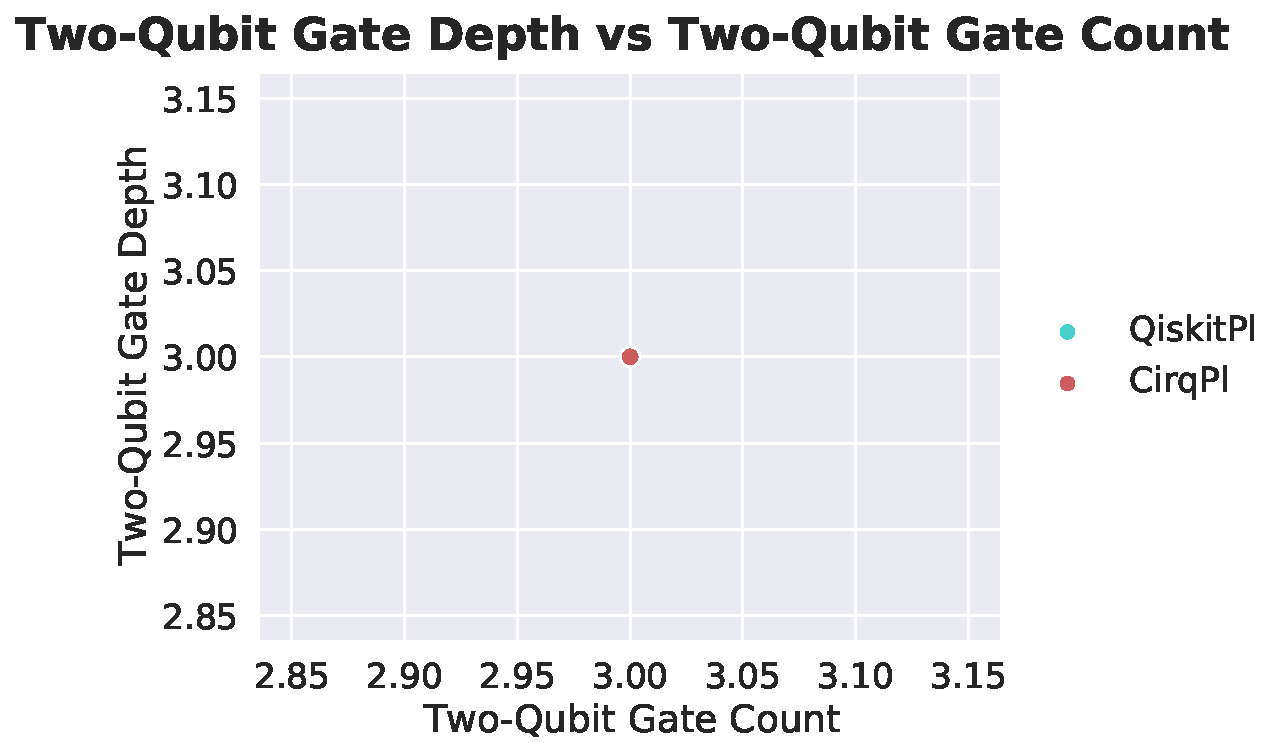
\includegraphics[width=0.4\textwidth]{/home/nathanschnitzer/arline_benchmarks/configs/compression/results/figures/kak/random_chain_clifford_t_2q_120/IbmAll2All2Q/scatter_two_qubit_gate_depth_vs_two_qubit_gate_count.pdf}%
\linebreak%
\caption{Cluster analytics for IbmAll2All2Q. Each point corresponds to an individual target
                    quantum circuit from the target generator.}%
\end{figure}

%
\clearpage%
\subsection*{Breakdown by individual circuits }%
\label{subsec:Breakdownbyindividualcircuits}%

%


\begin{figure}[h!]%
\centering%
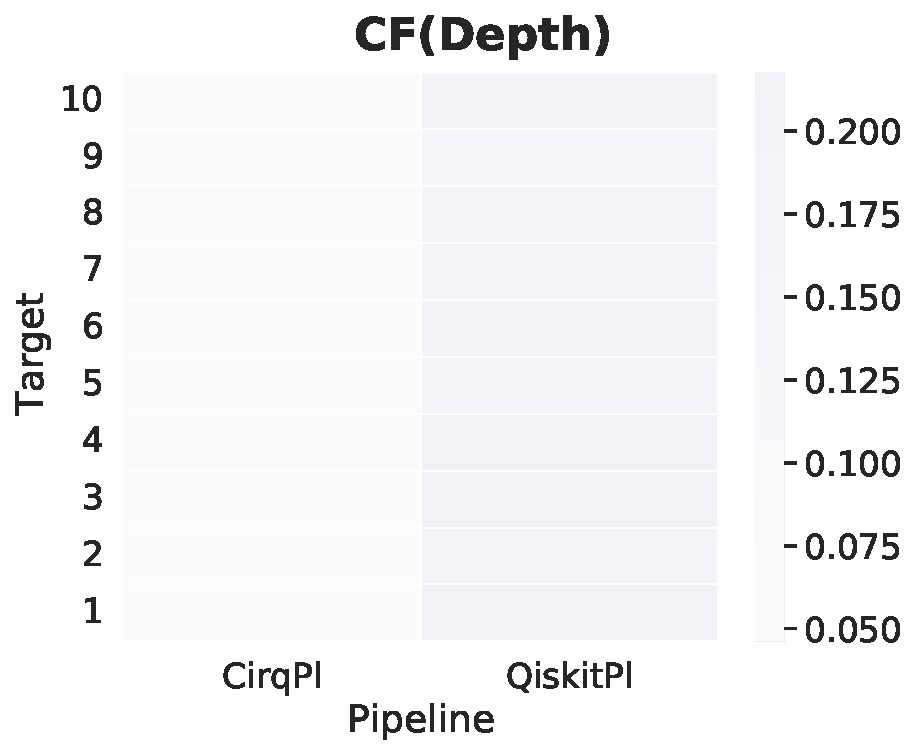
\includegraphics[width=0.4\textwidth]{/home/nathanschnitzer/arline_benchmarks/configs/compression/results/figures/kak/random_chain_clifford_t_2q_120/IbmAll2All2Q/comp_heatmap_depth_target_analysis_to_mapping_compression.pdf}%
\centering%
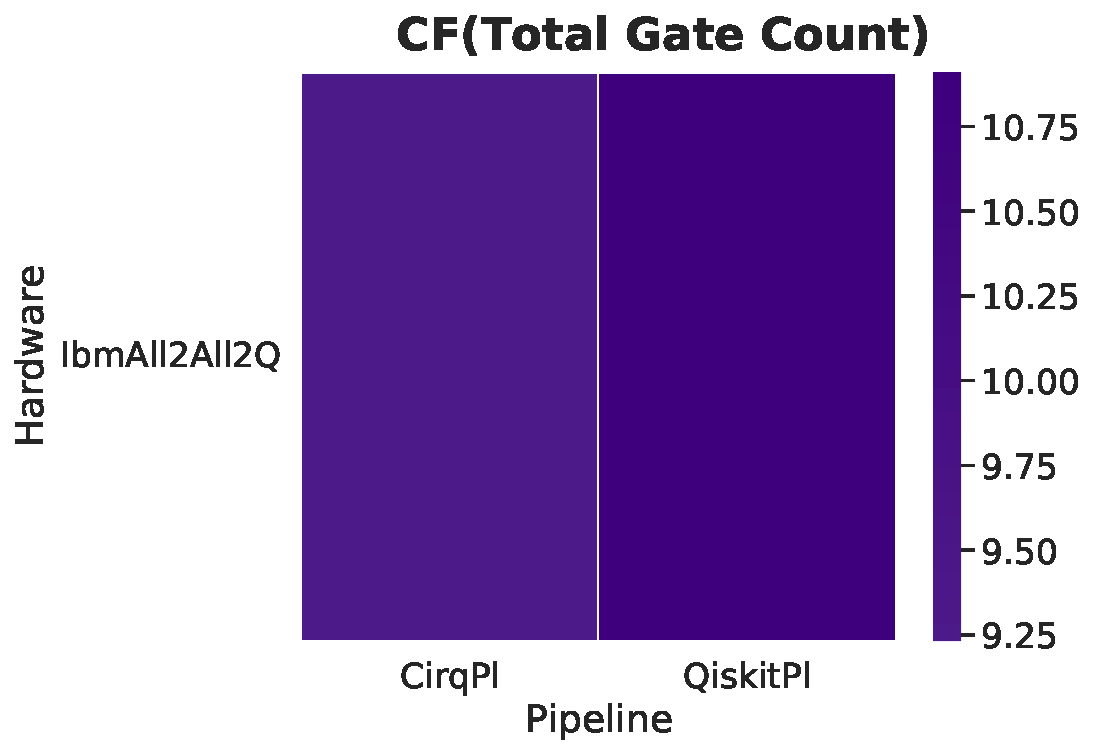
\includegraphics[width=0.4\textwidth]{/home/nathanschnitzer/arline_benchmarks/configs/compression/results/figures/kak/random_chain_clifford_t_2q_120/IbmAll2All2Q/comp_heatmap_total_gate_count_target_analysis_to_mapping_compression.pdf}%
\linebreak%
\centering%
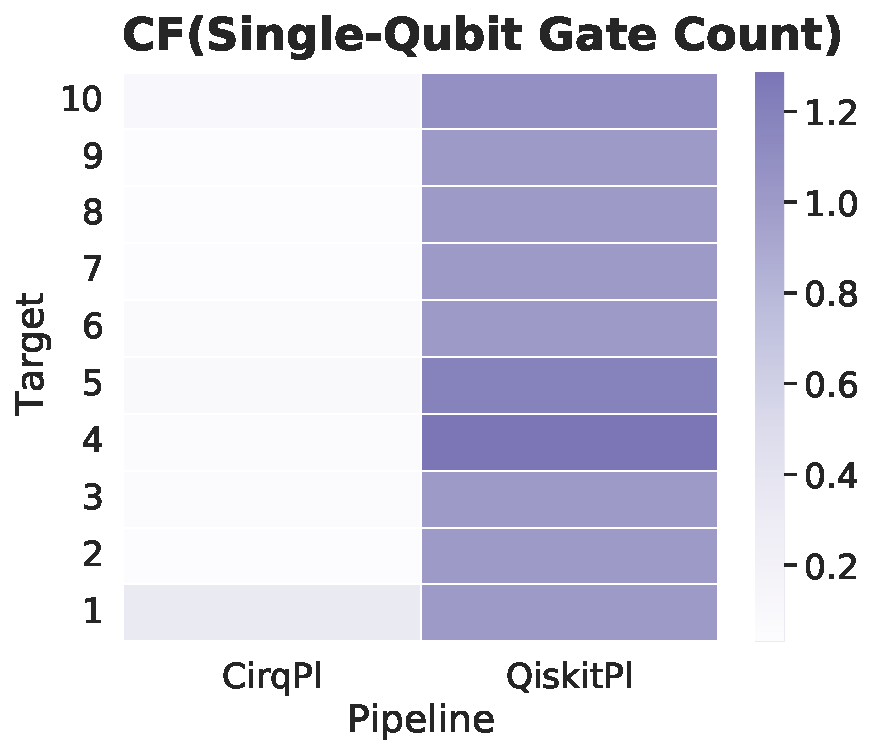
\includegraphics[width=0.4\textwidth]{/home/nathanschnitzer/arline_benchmarks/configs/compression/results/figures/kak/random_chain_clifford_t_2q_120/IbmAll2All2Q/comp_heatmap_single_qubit_gate_count_target_analysis_to_mapping_compression.pdf}%
\centering%
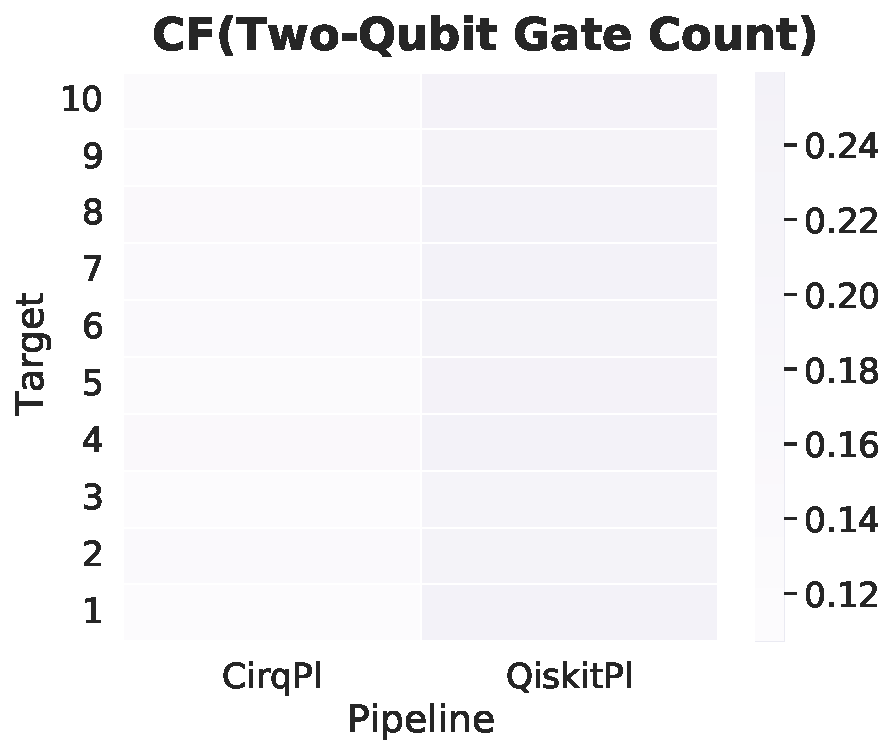
\includegraphics[width=0.4\textwidth]{/home/nathanschnitzer/arline_benchmarks/configs/compression/results/figures/kak/random_chain_clifford_t_2q_120/IbmAll2All2Q/comp_heatmap_two_qubit_gate_count_target_analysis_to_mapping_compression.pdf}%
\linebreak%
\centering%
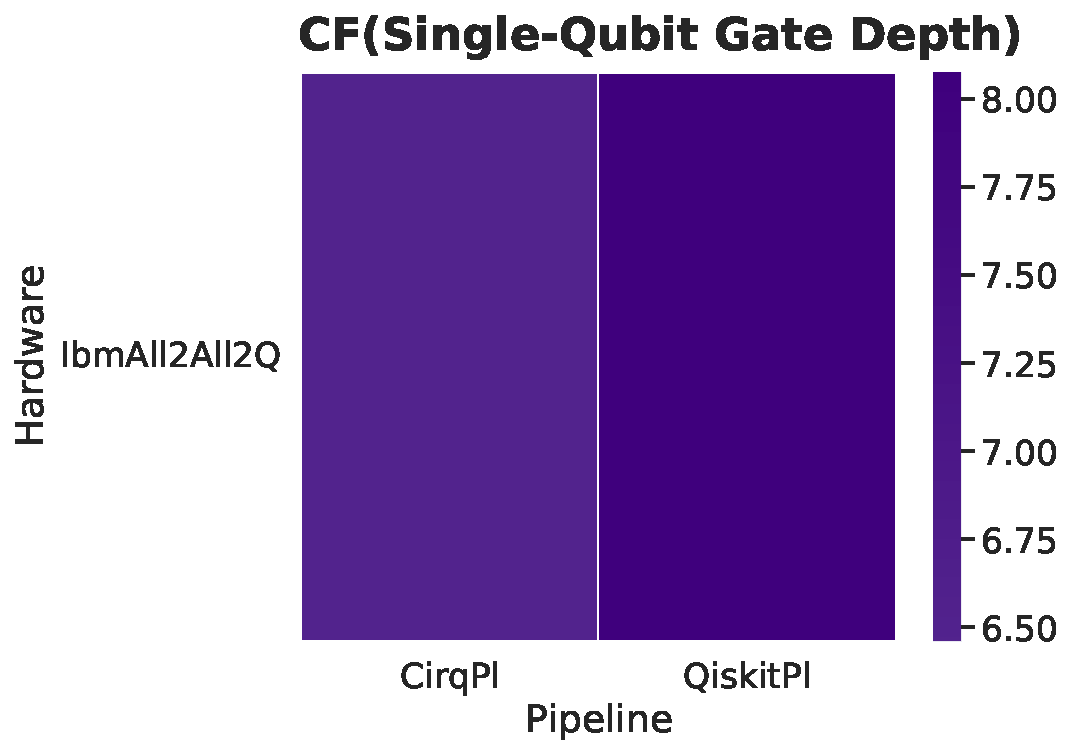
\includegraphics[width=0.4\textwidth]{/home/nathanschnitzer/arline_benchmarks/configs/compression/results/figures/kak/random_chain_clifford_t_2q_120/IbmAll2All2Q/comp_heatmap_single_qubit_gate_depth_target_analysis_to_mapping_compression.pdf}%
\centering%
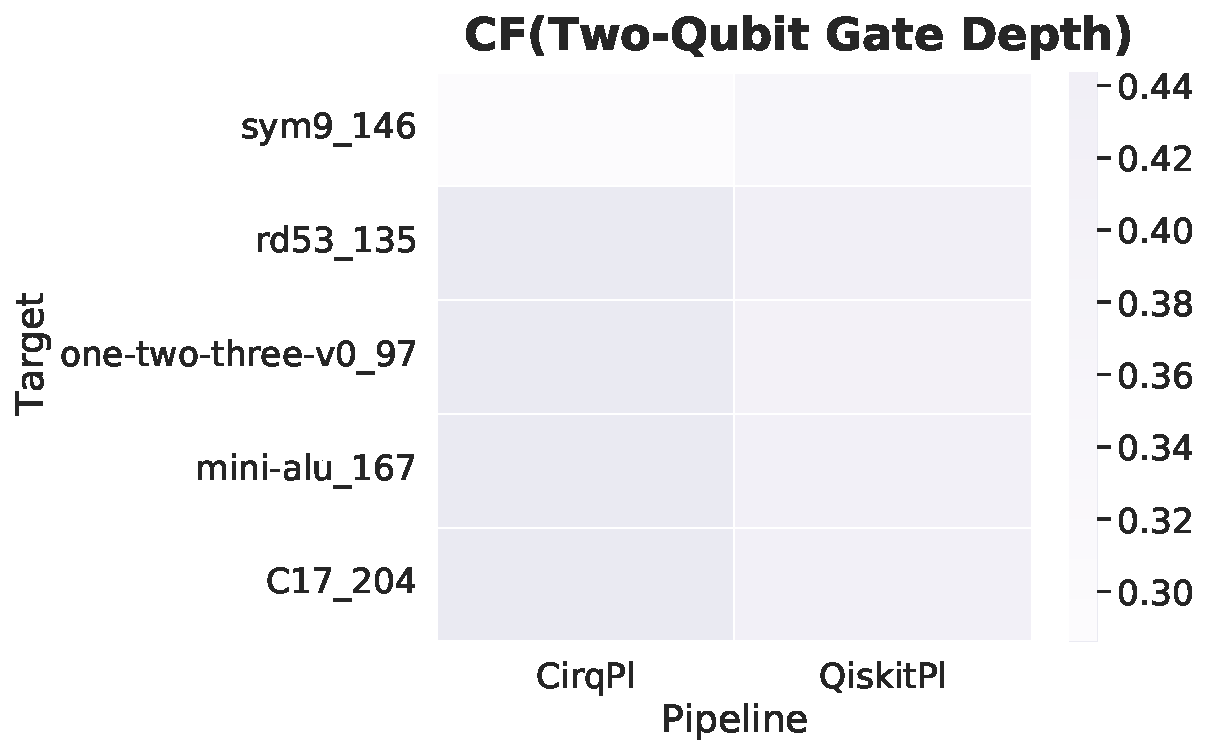
\includegraphics[width=0.4\textwidth]{/home/nathanschnitzer/arline_benchmarks/configs/compression/results/figures/kak/random_chain_clifford_t_2q_120/IbmAll2All2Q/comp_heatmap_two_qubit_gate_depth_target_analysis_to_mapping_compression.pdf}%
\linebreak%
\caption{Compression factor ($CF$) vs circuit for IbmAll2All2Q.}%
\end{figure}

%
\renewcommand{\arraystretch}{1.5}%
\begin{longtabu}{|X[3l]|X[l]|X[l]|X[l]|X[l]|X[l]|X[l]|}%
\hline%
\textbf{Metrics}&\multicolumn{3}{l|}{\textbf{Min}}&\multicolumn{3}{l|}{\textbf{Max}}\\%
\hline%
\rowcolor{lightgray}%
\textbf{}&\textbf{Pipeline}&\textbf{Circuit}&\textbf{Val}&\textbf{Pipeline}&\textbf{Circuit}&\textbf{Val}\\%
\hline%
\endhead%
\multicolumn{7}{|r|}{Continued on Next Page}\\%
\hline%
\endfoot%
\endlastfoot%
Depth&QiskitPl&6&5&CirqPl&1&8\\%
\hline%
Total Gate Count&QiskitPl&6&8&CirqPl&1&13\\%
\hline%
Single{-}Qubit Gate Count&QiskitPl&6&6&CirqPl&1&10\\%
\hline%
Two{-}Qubit Gate Count&QiskitPl&6&2&QiskitPl&1&3\\%
\hline%
Single{-}Qubit Gate Depth&QiskitPl&6&3&CirqPl&1&5\\%
\hline%
Two{-}Qubit Gate Depth&QiskitPl&6&2&QiskitPl&1&3\\%
\hline%
Circuit Cost Function&QiskitPl&6&0.051&CirqPl&1&0.08\\%
\hline%
Execution Time&CirqPl&8&0.054&QiskitPl&10&0.184\\%
\hline%
\end{longtabu}%
\section{Hardware Comparison}%
\label{sec:HardwareComparison}%
This analysis is performed across all classes of target circuit.%
\renewcommand{\arraystretch}{1.5}%
\begin{longtabu}{|l|l|l|}%
\hline%
\rowcolor{lightgray}%
\textbf{Metrics}&\textbf{Min}&\textbf{Max}\\%
\hline%
\endhead%
\multicolumn{3}{|r|}{Continued on Next Page}\\%
\hline%
\endfoot%
\endlastfoot%
Depth&IbmAll2All2Q&IbmAll2All2Q\\%
\hline%
Total Gate Count&IbmAll2All2Q&IbmAll2All2Q\\%
\hline%
Single{-}Qubit Gate Count&IbmAll2All2Q&IbmAll2All2Q\\%
\hline%
Two{-}Qubit Gate Count&IbmAll2All2Q&IbmAll2All2Q\\%
\hline%
Single{-}Qubit Gate Depth&IbmAll2All2Q&IbmAll2All2Q\\%
\hline%
Two{-}Qubit Gate Depth&IbmAll2All2Q&IbmAll2All2Q\\%
\hline%
Circuit Cost Function&IbmAll2All2Q&IbmAll2All2Q\\%
\hline%
Execution Time&IbmAll2All2Q&IbmAll2All2Q\\%
\hline%
\end{longtabu}%


\begin{figure}[h!]%
\centering%
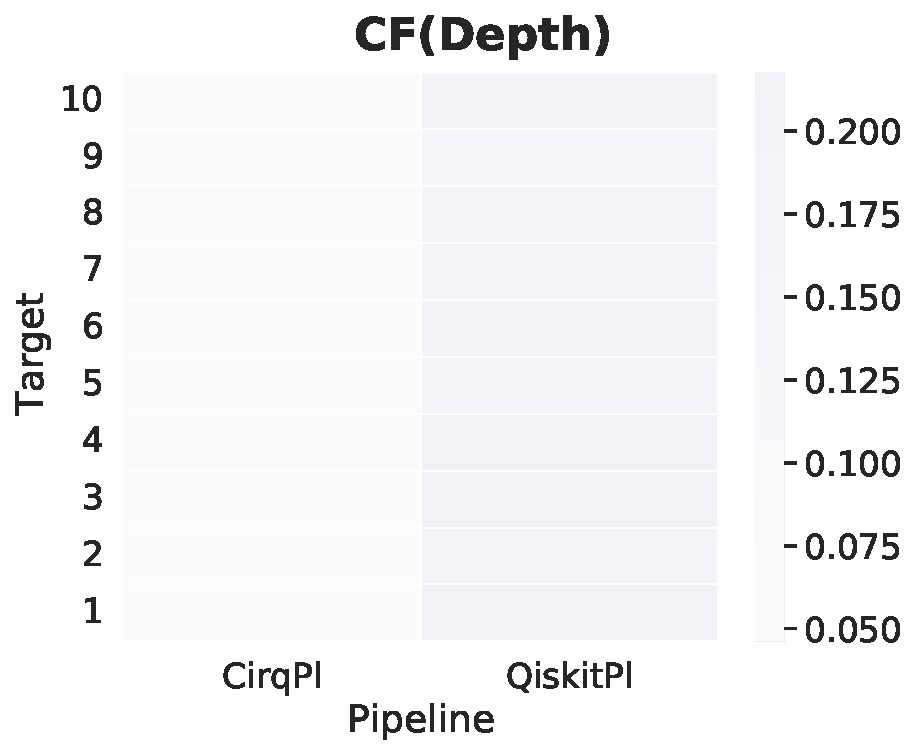
\includegraphics[width=0.4\textwidth]{/home/nathanschnitzer/arline_benchmarks/configs/compression/results/figures/kak/random_chain_clifford_t_2q_120/IbmAll2All2Q/comp_heatmap_depth_target_analysis_to_mapping_compression.pdf}%
\centering%
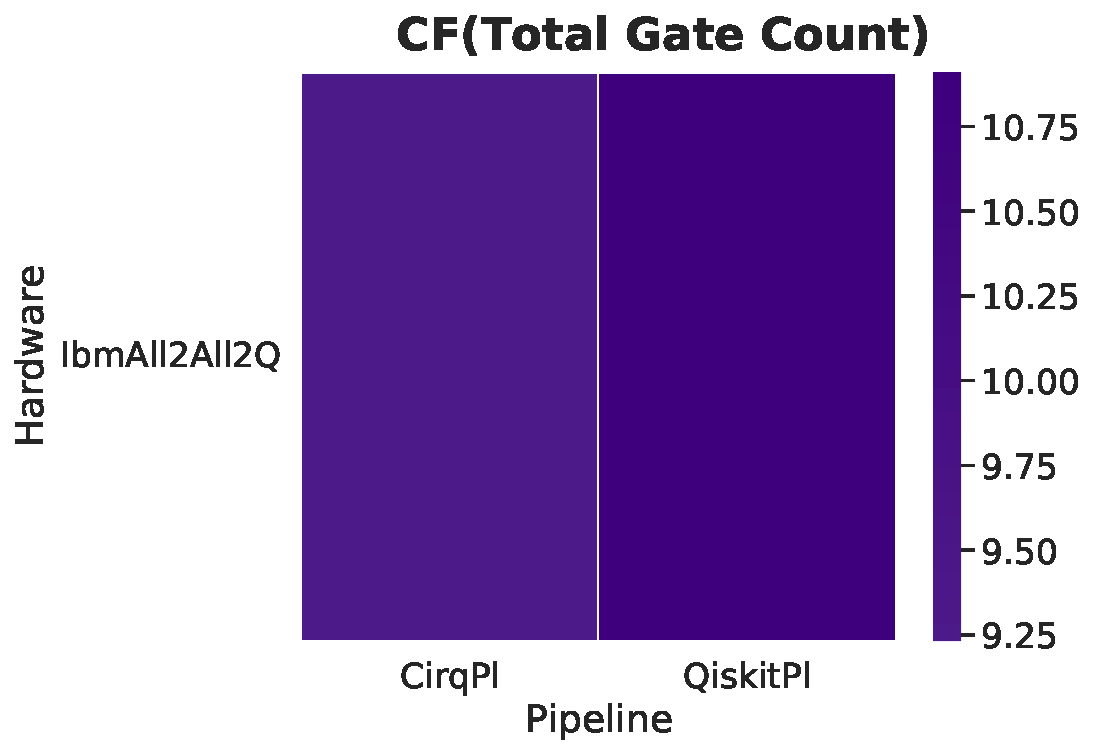
\includegraphics[width=0.4\textwidth]{/home/nathanschnitzer/arline_benchmarks/configs/compression/results/figures/kak/random_chain_clifford_t_2q_120/IbmAll2All2Q/comp_heatmap_total_gate_count_target_analysis_to_mapping_compression.pdf}%
\linebreak%
\centering%
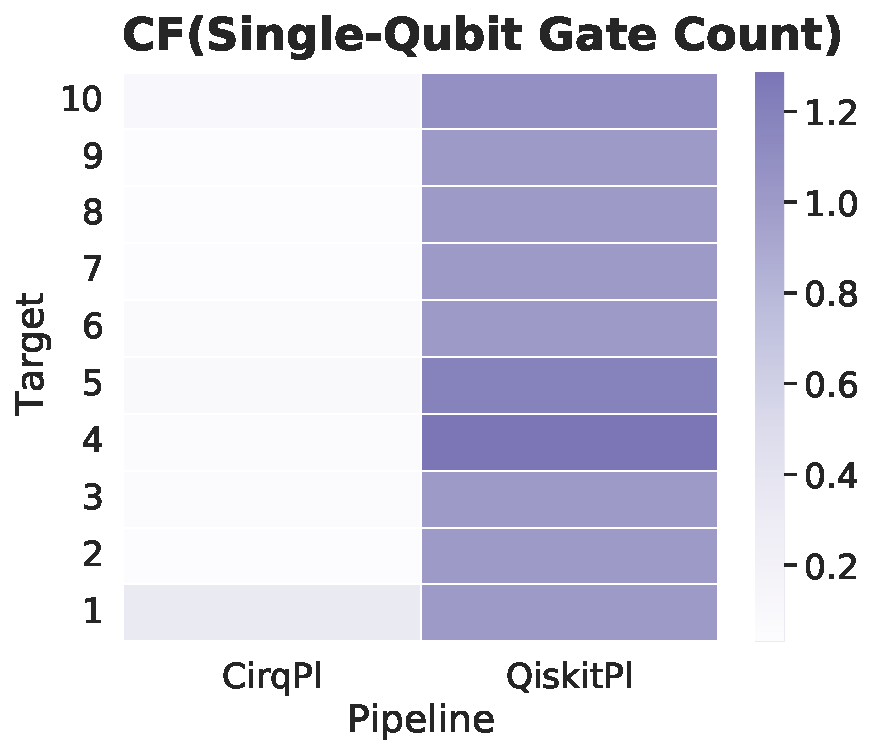
\includegraphics[width=0.4\textwidth]{/home/nathanschnitzer/arline_benchmarks/configs/compression/results/figures/kak/random_chain_clifford_t_2q_120/IbmAll2All2Q/comp_heatmap_single_qubit_gate_count_target_analysis_to_mapping_compression.pdf}%
\centering%
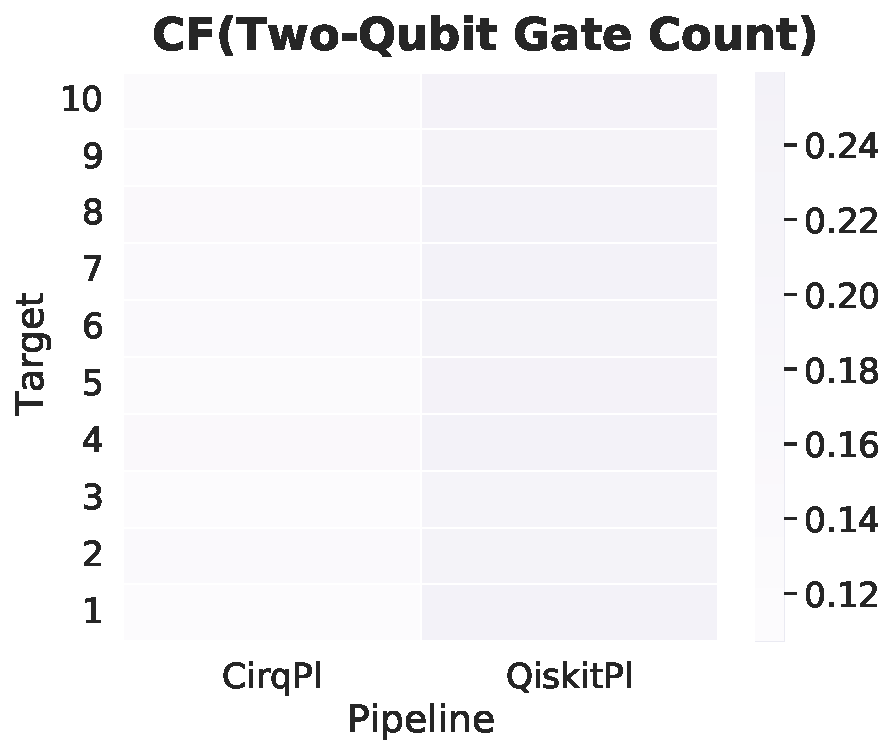
\includegraphics[width=0.4\textwidth]{/home/nathanschnitzer/arline_benchmarks/configs/compression/results/figures/kak/random_chain_clifford_t_2q_120/IbmAll2All2Q/comp_heatmap_two_qubit_gate_count_target_analysis_to_mapping_compression.pdf}%
\linebreak%
\centering%
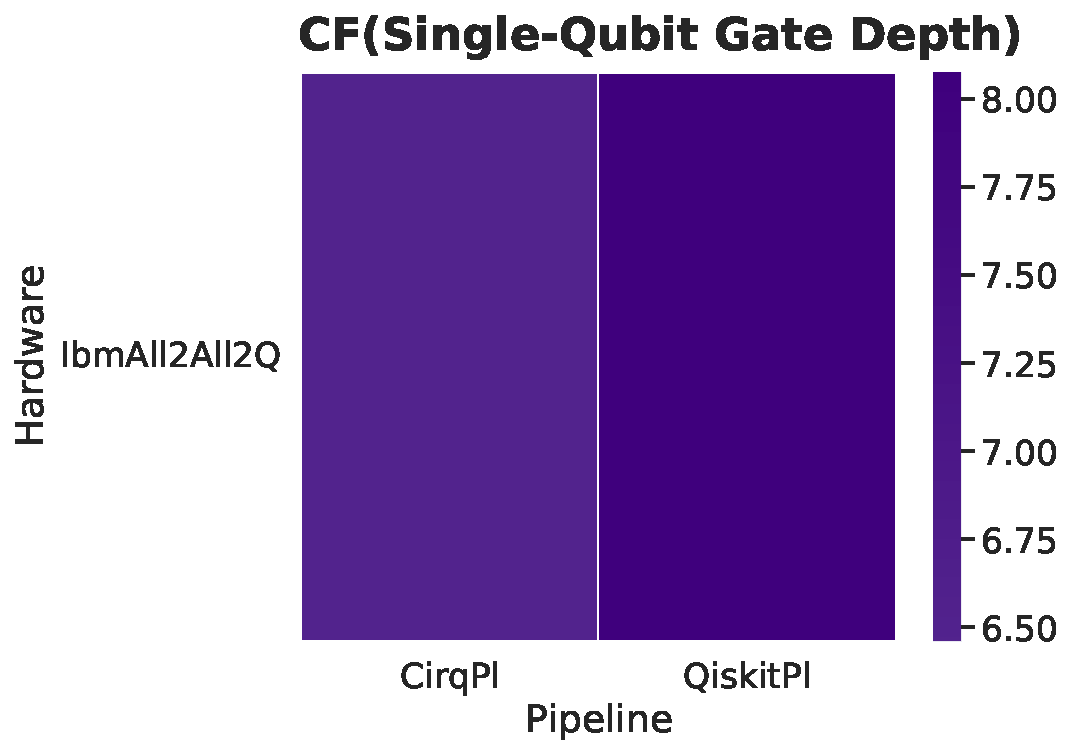
\includegraphics[width=0.4\textwidth]{/home/nathanschnitzer/arline_benchmarks/configs/compression/results/figures/kak/random_chain_clifford_t_2q_120/IbmAll2All2Q/comp_heatmap_single_qubit_gate_depth_target_analysis_to_mapping_compression.pdf}%
\centering%
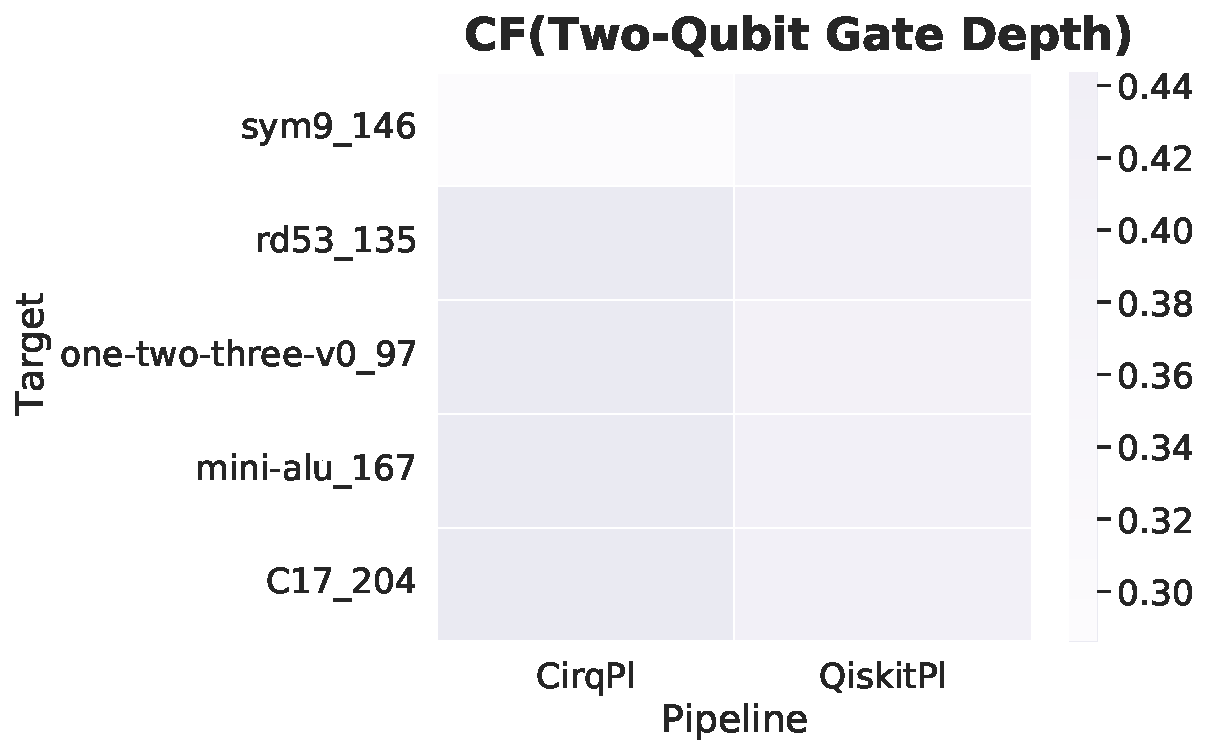
\includegraphics[width=0.4\textwidth]{/home/nathanschnitzer/arline_benchmarks/configs/compression/results/figures/kak/random_chain_clifford_t_2q_120/IbmAll2All2Q/comp_heatmap_two_qubit_gate_depth_target_analysis_to_mapping_compression.pdf}%
\linebreak%
\caption{Final circuit metrics after compilation vs hardware backend.}%
\end{figure}

%
\chapter{Target: Random Circuits from [CNOT, U$_3$] Gate Set}%
\label{chap:TargetRandomCircuitsfromCNOT,U3GateSet}%
\section{Hardware: IbmAll2All2Q}%
\label{sec:HardwareIbmAll2All2Q}%

%
\subsection*{Metrics for each stage of compilation pipeline and aggregate compression factor
                    (initial/final)}%
\label{subsec:Metricsforeachstageofcompilationpipelineandaggregatecompressionfactor(initial/final)}%

%
Note that in most cases single-qubit gate count and single-qubit gate compression factor
                have only limited meaning as a metric of compiler performance.This is because single-qubit
                gate count is very sensitive to the choice single-qubit basis gates (e.g. $U_3$ is
                equivalent to a combination of 3 rotation gates $R_x$, $R_y$ and $R_z$).%


\begin{figure}[h!]%
\centering%
\includegraphics[width=0.4\textwidth]{/home/nathanschnitzer/arline_benchmarks/configs/compression/results/figures/kak/random_chain_cnot_u3_2q_120/IbmAll2All2Q/bars_depth.pdf}%
\centering%
\includegraphics[width=0.4\textwidth]{/home/nathanschnitzer/arline_benchmarks/configs/compression/results/figures/kak/random_chain_cnot_u3_2q_120/IbmAll2All2Q/bars_total_gate_count.pdf}%
\linebreak%
\centering%
\includegraphics[width=0.4\textwidth]{/home/nathanschnitzer/arline_benchmarks/configs/compression/results/figures/kak/random_chain_cnot_u3_2q_120/IbmAll2All2Q/bars_single_qubit_gate_count.pdf}%
\centering%
\includegraphics[width=0.4\textwidth]{/home/nathanschnitzer/arline_benchmarks/configs/compression/results/figures/kak/random_chain_cnot_u3_2q_120/IbmAll2All2Q/bars_two_qubit_gate_count.pdf}%
\linebreak%
\centering%
\includegraphics[width=0.4\textwidth]{/home/nathanschnitzer/arline_benchmarks/configs/compression/results/figures/kak/random_chain_cnot_u3_2q_120/IbmAll2All2Q/bars_single_qubit_gate_depth.pdf}%
\centering%
\includegraphics[width=0.4\textwidth]{/home/nathanschnitzer/arline_benchmarks/configs/compression/results/figures/kak/random_chain_cnot_u3_2q_120/IbmAll2All2Q/bars_two_qubit_gate_depth.pdf}%
\linebreak%
\caption{Circuits metrics for each compilation pipeline stage for IbmAll2All2Q.}%
\end{figure}

%


\begin{figure}[h!]%
\centering%
\includegraphics[width=0.4\textwidth]{/home/nathanschnitzer/arline_benchmarks/configs/compression/results/figures/kak/random_chain_cnot_u3_2q_120/IbmAll2All2Q/bars_circuit_cost_function.pdf}%
\caption{Circuit cost function for IbmAll2All2Q.}%
\end{figure}

%


\begin{figure}[h!]%
\centering%
\includegraphics[width=0.4\textwidth]{/home/nathanschnitzer/arline_benchmarks/configs/compression/results/figures/kak/random_chain_cnot_u3_2q_120/IbmAll2All2Q/compression_target_analysis_to_mapping_compression.pdf}%
\centering%
\includegraphics[width=0.4\textwidth]{/home/nathanschnitzer/arline_benchmarks/configs/compression/results/figures/kak/random_chain_cnot_u3_2q_120/IbmAll2All2Q/comp_radar_target_analysis_to_mapping_compression.pdf}%
\caption{Compression factor ($CF$) between target and final compilation stage for IbmAll2All2Q
                        (histogram and radar plot).
                        }%
\end{figure}

%
\clearpage%
\subsection*{Gate composition for each compilation pipeline stage}%
\label{subsec:Gatecompositionforeachcompilationpipelinestage}%

%


\begin{figure}[h!]%
\centering%
\includegraphics[width=0.4\textwidth]{/home/nathanschnitzer/arline_benchmarks/configs/compression/results/figures/kak/random_chain_cnot_u3_2q_120/IbmAll2All2Q/gate_composition_heatmap_qiskitpl.pdf}%
\centering%
\includegraphics[width=0.4\textwidth]{/home/nathanschnitzer/arline_benchmarks/configs/compression/results/figures/kak/random_chain_cnot_u3_2q_120/IbmAll2All2Q/gate_composition_heatmap_cirqpl.pdf}%
\linebreak%
\caption{Gate frequencies in each pipeline stage for IbmAll2All2Q.}%
\end{figure}

%
\subsection*{Execution time stats }%
\label{subsec:Executiontimestats}%

%
Here we present stats about execution time (in seconds)
                spent by frameworks for each compilation stage.%


\begin{figure}[h!]%
\centering%
\includegraphics[width=0.4\textwidth]{/home/nathanschnitzer/arline_benchmarks/configs/compression/results/figures/kak/random_chain_cnot_u3_2q_120/IbmAll2All2Q/bars_execution_time.pdf}%
\caption{Mean execution time of each compilation stage for IbmAll2All2Q.}%
\end{figure}

%
\subsection*{Summary stats (averaged over target circuits) by pipeline}%
\label{subsec:Summarystats(averagedovertargetcircuits)bypipeline}%

%
\renewcommand{\arraystretch}{1.5}%
\begin{longtabu}{|l|l|l|}%
\hline%
\rowcolor{lightgray}%
\textbf{Metrics}&\textbf{Min}&\textbf{Max}\\%
\hline%
\endhead%
\multicolumn{3}{|r|}{Continued on Next Page}\\%
\hline%
\endfoot%
\endlastfoot%
Depth&QiskitPl&CirqPl\\%
\hline%
Total Gate Count&QiskitPl&CirqPl\\%
\hline%
Single{-}Qubit Gate Count&QiskitPl&CirqPl\\%
\hline%
Two{-}Qubit Gate Count&CirqPl&CirqPl\\%
\hline%
Single{-}Qubit Gate Depth&QiskitPl&CirqPl\\%
\hline%
Two{-}Qubit Gate Depth&CirqPl&CirqPl\\%
\hline%
Circuit Cost Function&QiskitPl&CirqPl\\%
\hline%
Execution Time&QiskitPl&CirqPl\\%
\hline%
\end{longtabu}%
\subsection*{Cluster analytics }%
\label{subsec:Clusteranalytics}%

%
Scatter plots with axes representing: depth, (input/output) single-qubit gate count,
                (input/output) two-qubit gate count, (input/output) total gate count and execution time.%


\begin{figure}[h!]%
\centering%
\includegraphics[width=0.4\textwidth]{/home/nathanschnitzer/arline_benchmarks/configs/compression/results/figures/kak/random_chain_cnot_u3_2q_120/IbmAll2All2Q/scatter_total_gate_count_vs_depth.pdf}%
\centering%
\includegraphics[width=0.4\textwidth]{/home/nathanschnitzer/arline_benchmarks/configs/compression/results/figures/kak/random_chain_cnot_u3_2q_120/IbmAll2All2Q/scatter_two_qubit_gate_count_vs_depth.pdf}%
\linebreak%
\centering%
\includegraphics[width=0.4\textwidth]{/home/nathanschnitzer/arline_benchmarks/configs/compression/results/figures/kak/random_chain_cnot_u3_2q_120/IbmAll2All2Q/scatter_two_qubit_gate_count_vs_single_qubit_gate_count.pdf}%
\centering%
\includegraphics[width=0.4\textwidth]{/home/nathanschnitzer/arline_benchmarks/configs/compression/results/figures/kak/random_chain_cnot_u3_2q_120/IbmAll2All2Q/scatter_total_execution_time_vs_total_gate_count.pdf}%
\linebreak%
\centering%
\includegraphics[width=0.4\textwidth]{/home/nathanschnitzer/arline_benchmarks/configs/compression/results/figures/kak/random_chain_cnot_u3_2q_120/IbmAll2All2Q/scatter_single_qubit_gate_depth_vs_single_qubit_gate_count.pdf}%
\centering%
\includegraphics[width=0.4\textwidth]{/home/nathanschnitzer/arline_benchmarks/configs/compression/results/figures/kak/random_chain_cnot_u3_2q_120/IbmAll2All2Q/scatter_two_qubit_gate_depth_vs_two_qubit_gate_count.pdf}%
\linebreak%
\caption{Cluster analytics for IbmAll2All2Q. Each point corresponds to an individual target
                    quantum circuit from the target generator.}%
\end{figure}

%
\clearpage%
\subsection*{Breakdown by individual circuits }%
\label{subsec:Breakdownbyindividualcircuits}%

%


\begin{figure}[h!]%
\centering%
\includegraphics[width=0.4\textwidth]{/home/nathanschnitzer/arline_benchmarks/configs/compression/results/figures/kak/random_chain_cnot_u3_2q_120/IbmAll2All2Q/comp_heatmap_depth_target_analysis_to_mapping_compression.pdf}%
\centering%
\includegraphics[width=0.4\textwidth]{/home/nathanschnitzer/arline_benchmarks/configs/compression/results/figures/kak/random_chain_cnot_u3_2q_120/IbmAll2All2Q/comp_heatmap_total_gate_count_target_analysis_to_mapping_compression.pdf}%
\linebreak%
\centering%
\includegraphics[width=0.4\textwidth]{/home/nathanschnitzer/arline_benchmarks/configs/compression/results/figures/kak/random_chain_cnot_u3_2q_120/IbmAll2All2Q/comp_heatmap_single_qubit_gate_count_target_analysis_to_mapping_compression.pdf}%
\centering%
\includegraphics[width=0.4\textwidth]{/home/nathanschnitzer/arline_benchmarks/configs/compression/results/figures/kak/random_chain_cnot_u3_2q_120/IbmAll2All2Q/comp_heatmap_two_qubit_gate_count_target_analysis_to_mapping_compression.pdf}%
\linebreak%
\centering%
\includegraphics[width=0.4\textwidth]{/home/nathanschnitzer/arline_benchmarks/configs/compression/results/figures/kak/random_chain_cnot_u3_2q_120/IbmAll2All2Q/comp_heatmap_single_qubit_gate_depth_target_analysis_to_mapping_compression.pdf}%
\centering%
\includegraphics[width=0.4\textwidth]{/home/nathanschnitzer/arline_benchmarks/configs/compression/results/figures/kak/random_chain_cnot_u3_2q_120/IbmAll2All2Q/comp_heatmap_two_qubit_gate_depth_target_analysis_to_mapping_compression.pdf}%
\linebreak%
\caption{Compression factor ($CF$) vs circuit for IbmAll2All2Q.}%
\end{figure}

%
\renewcommand{\arraystretch}{1.5}%
\begin{longtabu}{|X[3l]|X[l]|X[l]|X[l]|X[l]|X[l]|X[l]|}%
\hline%
\textbf{Metrics}&\multicolumn{3}{l|}{\textbf{Min}}&\multicolumn{3}{l|}{\textbf{Max}}\\%
\hline%
\rowcolor{lightgray}%
\textbf{}&\textbf{Pipeline}&\textbf{Circuit}&\textbf{Val}&\textbf{Pipeline}&\textbf{Circuit}&\textbf{Val}\\%
\hline%
\endhead%
\multicolumn{7}{|r|}{Continued on Next Page}\\%
\hline%
\endfoot%
\endlastfoot%
Depth&QiskitPl&1&7&CirqPl&1&8\\%
\hline%
Total Gate Count&QiskitPl&1&11&CirqPl&1&13\\%
\hline%
Single{-}Qubit Gate Count&QiskitPl&1&8&CirqPl&1&10\\%
\hline%
Two{-}Qubit Gate Count&QiskitPl&1&3&QiskitPl&1&3\\%
\hline%
Single{-}Qubit Gate Depth&QiskitPl&1&4&CirqPl&1&5\\%
\hline%
Two{-}Qubit Gate Depth&QiskitPl&1&3&QiskitPl&1&3\\%
\hline%
Circuit Cost Function&QiskitPl&1&0.073&CirqPl&1&0.08\\%
\hline%
Execution Time&QiskitPl&3&0.07&CirqPl&7&0.312\\%
\hline%
\end{longtabu}%
\section{Hardware Comparison}%
\label{sec:HardwareComparison}%
This analysis is performed across all classes of target circuit.%
\renewcommand{\arraystretch}{1.5}%
\begin{longtabu}{|l|l|l|}%
\hline%
\rowcolor{lightgray}%
\textbf{Metrics}&\textbf{Min}&\textbf{Max}\\%
\hline%
\endhead%
\multicolumn{3}{|r|}{Continued on Next Page}\\%
\hline%
\endfoot%
\endlastfoot%
Depth&IbmAll2All2Q&IbmAll2All2Q\\%
\hline%
Total Gate Count&IbmAll2All2Q&IbmAll2All2Q\\%
\hline%
Single{-}Qubit Gate Count&IbmAll2All2Q&IbmAll2All2Q\\%
\hline%
Two{-}Qubit Gate Count&IbmAll2All2Q&IbmAll2All2Q\\%
\hline%
Single{-}Qubit Gate Depth&IbmAll2All2Q&IbmAll2All2Q\\%
\hline%
Two{-}Qubit Gate Depth&IbmAll2All2Q&IbmAll2All2Q\\%
\hline%
Circuit Cost Function&IbmAll2All2Q&IbmAll2All2Q\\%
\hline%
Execution Time&IbmAll2All2Q&IbmAll2All2Q\\%
\hline%
\end{longtabu}%


\begin{figure}[h!]%
\centering%
\includegraphics[width=0.4\textwidth]{/home/nathanschnitzer/arline_benchmarks/configs/compression/results/figures/kak/random_chain_cnot_u3_2q_120/IbmAll2All2Q/comp_heatmap_depth_target_analysis_to_mapping_compression.pdf}%
\centering%
\includegraphics[width=0.4\textwidth]{/home/nathanschnitzer/arline_benchmarks/configs/compression/results/figures/kak/random_chain_cnot_u3_2q_120/IbmAll2All2Q/comp_heatmap_total_gate_count_target_analysis_to_mapping_compression.pdf}%
\linebreak%
\centering%
\includegraphics[width=0.4\textwidth]{/home/nathanschnitzer/arline_benchmarks/configs/compression/results/figures/kak/random_chain_cnot_u3_2q_120/IbmAll2All2Q/comp_heatmap_single_qubit_gate_count_target_analysis_to_mapping_compression.pdf}%
\centering%
\includegraphics[width=0.4\textwidth]{/home/nathanschnitzer/arline_benchmarks/configs/compression/results/figures/kak/random_chain_cnot_u3_2q_120/IbmAll2All2Q/comp_heatmap_two_qubit_gate_count_target_analysis_to_mapping_compression.pdf}%
\linebreak%
\centering%
\includegraphics[width=0.4\textwidth]{/home/nathanschnitzer/arline_benchmarks/configs/compression/results/figures/kak/random_chain_cnot_u3_2q_120/IbmAll2All2Q/comp_heatmap_single_qubit_gate_depth_target_analysis_to_mapping_compression.pdf}%
\centering%
\includegraphics[width=0.4\textwidth]{/home/nathanschnitzer/arline_benchmarks/configs/compression/results/figures/kak/random_chain_cnot_u3_2q_120/IbmAll2All2Q/comp_heatmap_two_qubit_gate_depth_target_analysis_to_mapping_compression.pdf}%
\linebreak%
\caption{Final circuit metrics after compilation vs hardware backend.}%
\end{figure}

%
\chapter{Quick Summary}%
\label{chap:QuickSummary}%
\section{Aggregate Multi{-}Factor Comparison}%
\label{sec:AggregateMulti{-}FactorComparison}%
This analysis is performed across all compilation frameworks, target circuits and hardware.
                        From this result, we can deduce the degree of compressibility of different target
                        circuits. \bigskip

                        \noindent{Note that in most cases single-qubit gate count and single-qubit gate compression
                        factor have only limited meaning as a metric of compiler performance. This is because
                        single-qubit gate count is very sensitive to the choice single-qubit basis gates
                        (e.g. $U_3$ is equivalent to a combination of 3 rotation gates $R_x$, $R_y$ and $R_z$).}
                        %


\begin{figure}[h!]%
\centering%
\includegraphics[width=0.45\textwidth]{/home/nathanschnitzer/arline_benchmarks/configs/compression/results/figures/multiqubit/comp_radar_target_analysis_to_mapping_compression_grid.pdf}%
\caption{Aggregate multi-factor comparison of compilation frameworks: compression factor
                                ($CF$) across various features. Columns correspond to specific target circuit classes,
                                and row correspond to different hardware architectures. Better performance corresponds
                                to a larger polygon area.}%
\end{figure}

%
\chapter{Target: Random Circuits from [Clifford + T] Gate Set}%
\label{chap:TargetRandomCircuitsfromClifford+TGateSet}%
\section{Hardware: IbmRueschlikonSymmetrical16Q}%
\label{sec:HardwareIbmRueschlikonSymmetrical16Q}%

%
\subsection*{Metrics for each stage of compilation pipeline and aggregate compression factor
                    (initial/final)}%
\label{subsec:Metricsforeachstageofcompilationpipelineandaggregatecompressionfactor(initial/final)}%

%
Note that in most cases single-qubit gate count and single-qubit gate compression factor
                have only limited meaning as a metric of compiler performance.This is because single-qubit
                gate count is very sensitive to the choice single-qubit basis gates (e.g. $U_3$ is
                equivalent to a combination of 3 rotation gates $R_x$, $R_y$ and $R_z$).%


\begin{figure}[h!]%
\centering%
\includegraphics[width=0.4\textwidth]{/home/nathanschnitzer/arline_benchmarks/configs/compression/results/figures/multiqubit/random_chain_clifford_t_16q_120/IbmRueschlikonSymmetrical16Q/bars_depth.pdf}%
\centering%
\includegraphics[width=0.4\textwidth]{/home/nathanschnitzer/arline_benchmarks/configs/compression/results/figures/multiqubit/random_chain_clifford_t_16q_120/IbmRueschlikonSymmetrical16Q/bars_total_gate_count.pdf}%
\linebreak%
\centering%
\includegraphics[width=0.4\textwidth]{/home/nathanschnitzer/arline_benchmarks/configs/compression/results/figures/multiqubit/random_chain_clifford_t_16q_120/IbmRueschlikonSymmetrical16Q/bars_single_qubit_gate_count.pdf}%
\centering%
\includegraphics[width=0.4\textwidth]{/home/nathanschnitzer/arline_benchmarks/configs/compression/results/figures/multiqubit/random_chain_clifford_t_16q_120/IbmRueschlikonSymmetrical16Q/bars_two_qubit_gate_count.pdf}%
\linebreak%
\centering%
\includegraphics[width=0.4\textwidth]{/home/nathanschnitzer/arline_benchmarks/configs/compression/results/figures/multiqubit/random_chain_clifford_t_16q_120/IbmRueschlikonSymmetrical16Q/bars_single_qubit_gate_depth.pdf}%
\centering%
\includegraphics[width=0.4\textwidth]{/home/nathanschnitzer/arline_benchmarks/configs/compression/results/figures/multiqubit/random_chain_clifford_t_16q_120/IbmRueschlikonSymmetrical16Q/bars_two_qubit_gate_depth.pdf}%
\linebreak%
\caption{Circuits metrics for each compilation pipeline stage for IbmRueschlikonSymmetrical16Q.}%
\end{figure}

%


\begin{figure}[h!]%
\centering%
\includegraphics[width=0.4\textwidth]{/home/nathanschnitzer/arline_benchmarks/configs/compression/results/figures/multiqubit/random_chain_clifford_t_16q_120/IbmRueschlikonSymmetrical16Q/bars_circuit_cost_function.pdf}%
\caption{Circuit cost function for IbmRueschlikonSymmetrical16Q.}%
\end{figure}

%


\begin{figure}[h!]%
\centering%
\includegraphics[width=0.4\textwidth]{/home/nathanschnitzer/arline_benchmarks/configs/compression/results/figures/multiqubit/random_chain_clifford_t_16q_120/IbmRueschlikonSymmetrical16Q/compression_target_analysis_to_mapping_compression.pdf}%
\centering%
\includegraphics[width=0.4\textwidth]{/home/nathanschnitzer/arline_benchmarks/configs/compression/results/figures/multiqubit/random_chain_clifford_t_16q_120/IbmRueschlikonSymmetrical16Q/comp_radar_target_analysis_to_mapping_compression.pdf}%
\caption{Compression factor ($CF$) between target and final compilation stage for IbmRueschlikonSymmetrical16Q
                        (histogram and radar plot).
                        }%
\end{figure}

%
\clearpage%
\subsection*{Gate composition for each compilation pipeline stage}%
\label{subsec:Gatecompositionforeachcompilationpipelinestage}%

%


\begin{figure}[h!]%
\centering%
\includegraphics[width=0.4\textwidth]{/home/nathanschnitzer/arline_benchmarks/configs/compression/results/figures/multiqubit/random_chain_clifford_t_16q_120/IbmRueschlikonSymmetrical16Q/gate_composition_heatmap_qiskitpl.pdf}%
\centering%
\includegraphics[width=0.4\textwidth]{/home/nathanschnitzer/arline_benchmarks/configs/compression/results/figures/multiqubit/random_chain_clifford_t_16q_120/IbmRueschlikonSymmetrical16Q/gate_composition_heatmap_cirqpl.pdf}%
\linebreak%
\caption{Gate frequencies in each pipeline stage for IbmRueschlikonSymmetrical16Q.}%
\end{figure}

%
\subsection*{Execution time stats }%
\label{subsec:Executiontimestats}%

%
Here we present stats about execution time (in seconds)
                spent by frameworks for each compilation stage.%


\begin{figure}[h!]%
\centering%
\includegraphics[width=0.4\textwidth]{/home/nathanschnitzer/arline_benchmarks/configs/compression/results/figures/multiqubit/random_chain_clifford_t_16q_120/IbmRueschlikonSymmetrical16Q/bars_execution_time.pdf}%
\caption{Mean execution time of each compilation stage for IbmRueschlikonSymmetrical16Q.}%
\end{figure}

%
\subsection*{Summary stats (averaged over target circuits) by pipeline}%
\label{subsec:Summarystats(averagedovertargetcircuits)bypipeline}%

%
\renewcommand{\arraystretch}{1.5}%
\begin{longtabu}{|l|l|l|}%
\hline%
\rowcolor{lightgray}%
\textbf{Metrics}&\textbf{Min}&\textbf{Max}\\%
\hline%
\endhead%
\multicolumn{3}{|r|}{Continued on Next Page}\\%
\hline%
\endfoot%
\endlastfoot%
Depth&QiskitPl&CirqPl\\%
\hline%
Total Gate Count&QiskitPl&CirqPl\\%
\hline%
Single{-}Qubit Gate Count&QiskitPl&CirqPl\\%
\hline%
Two{-}Qubit Gate Count&QiskitPl&CirqPl\\%
\hline%
Single{-}Qubit Gate Depth&QiskitPl&CirqPl\\%
\hline%
Two{-}Qubit Gate Depth&QiskitPl&CirqPl\\%
\hline%
Circuit Cost Function&QiskitPl&CirqPl\\%
\hline%
Execution Time&QiskitPl&CirqPl\\%
\hline%
\end{longtabu}%
\subsection*{Cluster analytics }%
\label{subsec:Clusteranalytics}%

%
Scatter plots with axes representing: depth, (input/output) single-qubit gate count,
                (input/output) two-qubit gate count, (input/output) total gate count and execution time.%


\begin{figure}[h!]%
\centering%
\includegraphics[width=0.4\textwidth]{/home/nathanschnitzer/arline_benchmarks/configs/compression/results/figures/multiqubit/random_chain_clifford_t_16q_120/IbmRueschlikonSymmetrical16Q/scatter_total_gate_count_vs_depth.pdf}%
\centering%
\includegraphics[width=0.4\textwidth]{/home/nathanschnitzer/arline_benchmarks/configs/compression/results/figures/multiqubit/random_chain_clifford_t_16q_120/IbmRueschlikonSymmetrical16Q/scatter_two_qubit_gate_count_vs_depth.pdf}%
\linebreak%
\centering%
\includegraphics[width=0.4\textwidth]{/home/nathanschnitzer/arline_benchmarks/configs/compression/results/figures/multiqubit/random_chain_clifford_t_16q_120/IbmRueschlikonSymmetrical16Q/scatter_two_qubit_gate_count_vs_single_qubit_gate_count.pdf}%
\centering%
\includegraphics[width=0.4\textwidth]{/home/nathanschnitzer/arline_benchmarks/configs/compression/results/figures/multiqubit/random_chain_clifford_t_16q_120/IbmRueschlikonSymmetrical16Q/scatter_total_execution_time_vs_total_gate_count.pdf}%
\linebreak%
\centering%
\includegraphics[width=0.4\textwidth]{/home/nathanschnitzer/arline_benchmarks/configs/compression/results/figures/multiqubit/random_chain_clifford_t_16q_120/IbmRueschlikonSymmetrical16Q/scatter_single_qubit_gate_depth_vs_single_qubit_gate_count.pdf}%
\centering%
\includegraphics[width=0.4\textwidth]{/home/nathanschnitzer/arline_benchmarks/configs/compression/results/figures/multiqubit/random_chain_clifford_t_16q_120/IbmRueschlikonSymmetrical16Q/scatter_two_qubit_gate_depth_vs_two_qubit_gate_count.pdf}%
\linebreak%
\caption{Cluster analytics for IbmRueschlikonSymmetrical16Q. Each point corresponds to an individual target
                    quantum circuit from the target generator.}%
\end{figure}

%
\clearpage%
\subsection*{Breakdown by individual circuits }%
\label{subsec:Breakdownbyindividualcircuits}%

%


\begin{figure}[h!]%
\centering%
\includegraphics[width=0.4\textwidth]{/home/nathanschnitzer/arline_benchmarks/configs/compression/results/figures/multiqubit/random_chain_clifford_t_16q_120/IbmRueschlikonSymmetrical16Q/comp_heatmap_depth_target_analysis_to_mapping_compression.pdf}%
\centering%
\includegraphics[width=0.4\textwidth]{/home/nathanschnitzer/arline_benchmarks/configs/compression/results/figures/multiqubit/random_chain_clifford_t_16q_120/IbmRueschlikonSymmetrical16Q/comp_heatmap_total_gate_count_target_analysis_to_mapping_compression.pdf}%
\linebreak%
\centering%
\includegraphics[width=0.4\textwidth]{/home/nathanschnitzer/arline_benchmarks/configs/compression/results/figures/multiqubit/random_chain_clifford_t_16q_120/IbmRueschlikonSymmetrical16Q/comp_heatmap_single_qubit_gate_count_target_analysis_to_mapping_compression.pdf}%
\centering%
\includegraphics[width=0.4\textwidth]{/home/nathanschnitzer/arline_benchmarks/configs/compression/results/figures/multiqubit/random_chain_clifford_t_16q_120/IbmRueschlikonSymmetrical16Q/comp_heatmap_two_qubit_gate_count_target_analysis_to_mapping_compression.pdf}%
\linebreak%
\centering%
\includegraphics[width=0.4\textwidth]{/home/nathanschnitzer/arline_benchmarks/configs/compression/results/figures/multiqubit/random_chain_clifford_t_16q_120/IbmRueschlikonSymmetrical16Q/comp_heatmap_single_qubit_gate_depth_target_analysis_to_mapping_compression.pdf}%
\centering%
\includegraphics[width=0.4\textwidth]{/home/nathanschnitzer/arline_benchmarks/configs/compression/results/figures/multiqubit/random_chain_clifford_t_16q_120/IbmRueschlikonSymmetrical16Q/comp_heatmap_two_qubit_gate_depth_target_analysis_to_mapping_compression.pdf}%
\linebreak%
\caption{Compression factor ($CF$) vs circuit for IbmRueschlikonSymmetrical16Q.}%
\end{figure}

%
\renewcommand{\arraystretch}{1.5}%
\begin{longtabu}{|X[3l]|X[l]|X[l]|X[l]|X[l]|X[l]|X[l]|}%
\hline%
\textbf{Metrics}&\multicolumn{3}{l|}{\textbf{Min}}&\multicolumn{3}{l|}{\textbf{Max}}\\%
\hline%
\rowcolor{lightgray}%
\textbf{}&\textbf{Pipeline}&\textbf{Circuit}&\textbf{Val}&\textbf{Pipeline}&\textbf{Circuit}&\textbf{Val}\\%
\hline%
\endhead%
\multicolumn{7}{|r|}{Continued on Next Page}\\%
\hline%
\endfoot%
\endlastfoot%
Depth&QiskitPl&1&145&CirqPl&7&743\\%
\hline%
Total Gate Count&QiskitPl&1&403&CirqPl&1&2147\\%
\hline%
Single{-}Qubit Gate Count&QiskitPl&7&50&CirqPl&1&1382\\%
\hline%
Two{-}Qubit Gate Count&QiskitPl&1&323&CirqPl&1&765\\%
\hline%
Single{-}Qubit Gate Depth&QiskitPl&4&8&CirqPl&10&158\\%
\hline%
Two{-}Qubit Gate Depth&QiskitPl&1&130&CirqPl&7&383\\%
\hline%
Circuit Cost Function&QiskitPl&1&4.053&CirqPl&1&12.435\\%
\hline%
Execution Time&QiskitPl&1&0.71&CirqPl&1&9.678\\%
\hline%
\end{longtabu}%
\section{Hardware: IbmAll2All16Q}%
\label{sec:HardwareIbmAll2All16Q}%

%
\subsection*{Metrics for each stage of compilation pipeline and aggregate compression factor
                    (initial/final)}%
\label{subsec:Metricsforeachstageofcompilationpipelineandaggregatecompressionfactor(initial/final)}%

%
Note that in most cases single-qubit gate count and single-qubit gate compression factor
                have only limited meaning as a metric of compiler performance.This is because single-qubit
                gate count is very sensitive to the choice single-qubit basis gates (e.g. $U_3$ is
                equivalent to a combination of 3 rotation gates $R_x$, $R_y$ and $R_z$).%


\begin{figure}[h!]%
\centering%
\includegraphics[width=0.4\textwidth]{/home/nathanschnitzer/arline_benchmarks/configs/compression/results/figures/multiqubit/random_chain_clifford_t_16q_120/IbmAll2All16Q/bars_depth.pdf}%
\centering%
\includegraphics[width=0.4\textwidth]{/home/nathanschnitzer/arline_benchmarks/configs/compression/results/figures/multiqubit/random_chain_clifford_t_16q_120/IbmAll2All16Q/bars_total_gate_count.pdf}%
\linebreak%
\centering%
\includegraphics[width=0.4\textwidth]{/home/nathanschnitzer/arline_benchmarks/configs/compression/results/figures/multiqubit/random_chain_clifford_t_16q_120/IbmAll2All16Q/bars_single_qubit_gate_count.pdf}%
\centering%
\includegraphics[width=0.4\textwidth]{/home/nathanschnitzer/arline_benchmarks/configs/compression/results/figures/multiqubit/random_chain_clifford_t_16q_120/IbmAll2All16Q/bars_two_qubit_gate_count.pdf}%
\linebreak%
\centering%
\includegraphics[width=0.4\textwidth]{/home/nathanschnitzer/arline_benchmarks/configs/compression/results/figures/multiqubit/random_chain_clifford_t_16q_120/IbmAll2All16Q/bars_single_qubit_gate_depth.pdf}%
\centering%
\includegraphics[width=0.4\textwidth]{/home/nathanschnitzer/arline_benchmarks/configs/compression/results/figures/multiqubit/random_chain_clifford_t_16q_120/IbmAll2All16Q/bars_two_qubit_gate_depth.pdf}%
\linebreak%
\caption{Circuits metrics for each compilation pipeline stage for IbmAll2All16Q.}%
\end{figure}

%


\begin{figure}[h!]%
\centering%
\includegraphics[width=0.4\textwidth]{/home/nathanschnitzer/arline_benchmarks/configs/compression/results/figures/multiqubit/random_chain_clifford_t_16q_120/IbmAll2All16Q/bars_circuit_cost_function.pdf}%
\caption{Circuit cost function for IbmAll2All16Q.}%
\end{figure}

%


\begin{figure}[h!]%
\centering%
\includegraphics[width=0.4\textwidth]{/home/nathanschnitzer/arline_benchmarks/configs/compression/results/figures/multiqubit/random_chain_clifford_t_16q_120/IbmAll2All16Q/compression_target_analysis_to_mapping_compression.pdf}%
\centering%
\includegraphics[width=0.4\textwidth]{/home/nathanschnitzer/arline_benchmarks/configs/compression/results/figures/multiqubit/random_chain_clifford_t_16q_120/IbmAll2All16Q/comp_radar_target_analysis_to_mapping_compression.pdf}%
\caption{Compression factor ($CF$) between target and final compilation stage for IbmAll2All16Q
                        (histogram and radar plot).
                        }%
\end{figure}

%
\clearpage%
\subsection*{Gate composition for each compilation pipeline stage}%
\label{subsec:Gatecompositionforeachcompilationpipelinestage}%

%


\begin{figure}[h!]%
\centering%
\includegraphics[width=0.4\textwidth]{/home/nathanschnitzer/arline_benchmarks/configs/compression/results/figures/multiqubit/random_chain_clifford_t_16q_120/IbmAll2All16Q/gate_composition_heatmap_qiskitpl.pdf}%
\centering%
\includegraphics[width=0.4\textwidth]{/home/nathanschnitzer/arline_benchmarks/configs/compression/results/figures/multiqubit/random_chain_clifford_t_16q_120/IbmAll2All16Q/gate_composition_heatmap_cirqpl.pdf}%
\linebreak%
\caption{Gate frequencies in each pipeline stage for IbmAll2All16Q.}%
\end{figure}

%
\subsection*{Execution time stats }%
\label{subsec:Executiontimestats}%

%
Here we present stats about execution time (in seconds)
                spent by frameworks for each compilation stage.%


\begin{figure}[h!]%
\centering%
\includegraphics[width=0.4\textwidth]{/home/nathanschnitzer/arline_benchmarks/configs/compression/results/figures/multiqubit/random_chain_clifford_t_16q_120/IbmAll2All16Q/bars_execution_time.pdf}%
\caption{Mean execution time of each compilation stage for IbmAll2All16Q.}%
\end{figure}

%
\subsection*{Summary stats (averaged over target circuits) by pipeline}%
\label{subsec:Summarystats(averagedovertargetcircuits)bypipeline}%

%
\renewcommand{\arraystretch}{1.5}%
\begin{longtabu}{|l|l|l|}%
\hline%
\rowcolor{lightgray}%
\textbf{Metrics}&\textbf{Min}&\textbf{Max}\\%
\hline%
\endhead%
\multicolumn{3}{|r|}{Continued on Next Page}\\%
\hline%
\endfoot%
\endlastfoot%
Depth&QiskitPl&CirqPl\\%
\hline%
Total Gate Count&QiskitPl&CirqPl\\%
\hline%
Single{-}Qubit Gate Count&QiskitPl&CirqPl\\%
\hline%
Two{-}Qubit Gate Count&QiskitPl&CirqPl\\%
\hline%
Single{-}Qubit Gate Depth&QiskitPl&CirqPl\\%
\hline%
Two{-}Qubit Gate Depth&QiskitPl&CirqPl\\%
\hline%
Circuit Cost Function&QiskitPl&CirqPl\\%
\hline%
Execution Time&QiskitPl&CirqPl\\%
\hline%
\end{longtabu}%
\subsection*{Cluster analytics }%
\label{subsec:Clusteranalytics}%

%
Scatter plots with axes representing: depth, (input/output) single-qubit gate count,
                (input/output) two-qubit gate count, (input/output) total gate count and execution time.%


\begin{figure}[h!]%
\centering%
\includegraphics[width=0.4\textwidth]{/home/nathanschnitzer/arline_benchmarks/configs/compression/results/figures/multiqubit/random_chain_clifford_t_16q_120/IbmAll2All16Q/scatter_total_gate_count_vs_depth.pdf}%
\centering%
\includegraphics[width=0.4\textwidth]{/home/nathanschnitzer/arline_benchmarks/configs/compression/results/figures/multiqubit/random_chain_clifford_t_16q_120/IbmAll2All16Q/scatter_two_qubit_gate_count_vs_depth.pdf}%
\linebreak%
\centering%
\includegraphics[width=0.4\textwidth]{/home/nathanschnitzer/arline_benchmarks/configs/compression/results/figures/multiqubit/random_chain_clifford_t_16q_120/IbmAll2All16Q/scatter_two_qubit_gate_count_vs_single_qubit_gate_count.pdf}%
\centering%
\includegraphics[width=0.4\textwidth]{/home/nathanschnitzer/arline_benchmarks/configs/compression/results/figures/multiqubit/random_chain_clifford_t_16q_120/IbmAll2All16Q/scatter_total_execution_time_vs_total_gate_count.pdf}%
\linebreak%
\centering%
\includegraphics[width=0.4\textwidth]{/home/nathanschnitzer/arline_benchmarks/configs/compression/results/figures/multiqubit/random_chain_clifford_t_16q_120/IbmAll2All16Q/scatter_single_qubit_gate_depth_vs_single_qubit_gate_count.pdf}%
\centering%
\includegraphics[width=0.4\textwidth]{/home/nathanschnitzer/arline_benchmarks/configs/compression/results/figures/multiqubit/random_chain_clifford_t_16q_120/IbmAll2All16Q/scatter_two_qubit_gate_depth_vs_two_qubit_gate_count.pdf}%
\linebreak%
\caption{Cluster analytics for IbmAll2All16Q. Each point corresponds to an individual target
                    quantum circuit from the target generator.}%
\end{figure}

%
\clearpage%
\subsection*{Breakdown by individual circuits }%
\label{subsec:Breakdownbyindividualcircuits}%

%


\begin{figure}[h!]%
\centering%
\includegraphics[width=0.4\textwidth]{/home/nathanschnitzer/arline_benchmarks/configs/compression/results/figures/multiqubit/random_chain_clifford_t_16q_120/IbmAll2All16Q/comp_heatmap_depth_target_analysis_to_mapping_compression.pdf}%
\centering%
\includegraphics[width=0.4\textwidth]{/home/nathanschnitzer/arline_benchmarks/configs/compression/results/figures/multiqubit/random_chain_clifford_t_16q_120/IbmAll2All16Q/comp_heatmap_total_gate_count_target_analysis_to_mapping_compression.pdf}%
\linebreak%
\centering%
\includegraphics[width=0.4\textwidth]{/home/nathanschnitzer/arline_benchmarks/configs/compression/results/figures/multiqubit/random_chain_clifford_t_16q_120/IbmAll2All16Q/comp_heatmap_single_qubit_gate_count_target_analysis_to_mapping_compression.pdf}%
\centering%
\includegraphics[width=0.4\textwidth]{/home/nathanschnitzer/arline_benchmarks/configs/compression/results/figures/multiqubit/random_chain_clifford_t_16q_120/IbmAll2All16Q/comp_heatmap_two_qubit_gate_count_target_analysis_to_mapping_compression.pdf}%
\linebreak%
\centering%
\includegraphics[width=0.4\textwidth]{/home/nathanschnitzer/arline_benchmarks/configs/compression/results/figures/multiqubit/random_chain_clifford_t_16q_120/IbmAll2All16Q/comp_heatmap_single_qubit_gate_depth_target_analysis_to_mapping_compression.pdf}%
\centering%
\includegraphics[width=0.4\textwidth]{/home/nathanschnitzer/arline_benchmarks/configs/compression/results/figures/multiqubit/random_chain_clifford_t_16q_120/IbmAll2All16Q/comp_heatmap_two_qubit_gate_depth_target_analysis_to_mapping_compression.pdf}%
\linebreak%
\caption{Compression factor ($CF$) vs circuit for IbmAll2All16Q.}%
\end{figure}

%
\renewcommand{\arraystretch}{1.5}%
\begin{longtabu}{|X[3l]|X[l]|X[l]|X[l]|X[l]|X[l]|X[l]|}%
\hline%
\textbf{Metrics}&\multicolumn{3}{l|}{\textbf{Min}}&\multicolumn{3}{l|}{\textbf{Max}}\\%
\hline%
\rowcolor{lightgray}%
\textbf{}&\textbf{Pipeline}&\textbf{Circuit}&\textbf{Val}&\textbf{Pipeline}&\textbf{Circuit}&\textbf{Val}\\%
\hline%
\endhead%
\multicolumn{7}{|r|}{Continued on Next Page}\\%
\hline%
\endfoot%
\endlastfoot%
Depth&QiskitPl&9&28&CirqPl&4&62\\%
\hline%
Total Gate Count&QiskitPl&3&103&CirqPl&7&224\\%
\hline%
Single{-}Qubit Gate Count&QiskitPl&4&19&CirqPl&1&138\\%
\hline%
Two{-}Qubit Gate Count&QiskitPl&3&75&CirqPl&4&93\\%
\hline%
Single{-}Qubit Gate Depth&QiskitPl&4&2&CirqPl&1&15\\%
\hline%
Two{-}Qubit Gate Depth&QiskitPl&1&25&CirqPl&4&38\\%
\hline%
Circuit Cost Function&QiskitPl&3&0.942&CirqPl&4&1.371\\%
\hline%
Execution Time&QiskitPl&9&0.174&CirqPl&3&0.696\\%
\hline%
\end{longtabu}%
\section{Hardware Comparison}%
\label{sec:HardwareComparison}%
This analysis is performed across all classes of target circuit.%
\renewcommand{\arraystretch}{1.5}%
\begin{longtabu}{|l|l|l|}%
\hline%
\rowcolor{lightgray}%
\textbf{Metrics}&\textbf{Min}&\textbf{Max}\\%
\hline%
\endhead%
\multicolumn{3}{|r|}{Continued on Next Page}\\%
\hline%
\endfoot%
\endlastfoot%
Depth&IbmAll2All16Q&IbmAll2All16Q\\%
\hline%
Total Gate Count&IbmAll2All16Q&IbmAll2All16Q\\%
\hline%
Single{-}Qubit Gate Count&IbmAll2All16Q&IbmAll2All16Q\\%
\hline%
Two{-}Qubit Gate Count&IbmAll2All16Q&IbmAll2All16Q\\%
\hline%
Single{-}Qubit Gate Depth&IbmAll2All16Q&IbmAll2All16Q\\%
\hline%
Two{-}Qubit Gate Depth&IbmAll2All16Q&IbmAll2All16Q\\%
\hline%
Circuit Cost Function&IbmAll2All16Q&IbmAll2All16Q\\%
\hline%
Execution Time&IbmAll2All16Q&IbmAll2All16Q\\%
\hline%
\end{longtabu}%


\begin{figure}[h!]%
\centering%
\includegraphics[width=0.4\textwidth]{/home/nathanschnitzer/arline_benchmarks/configs/compression/results/figures/multiqubit/random_chain_clifford_t_16q_120/IbmAll2All16Q/comp_heatmap_depth_target_analysis_to_mapping_compression.pdf}%
\centering%
\includegraphics[width=0.4\textwidth]{/home/nathanschnitzer/arline_benchmarks/configs/compression/results/figures/multiqubit/random_chain_clifford_t_16q_120/IbmAll2All16Q/comp_heatmap_total_gate_count_target_analysis_to_mapping_compression.pdf}%
\linebreak%
\centering%
\includegraphics[width=0.4\textwidth]{/home/nathanschnitzer/arline_benchmarks/configs/compression/results/figures/multiqubit/random_chain_clifford_t_16q_120/IbmAll2All16Q/comp_heatmap_single_qubit_gate_count_target_analysis_to_mapping_compression.pdf}%
\centering%
\includegraphics[width=0.4\textwidth]{/home/nathanschnitzer/arline_benchmarks/configs/compression/results/figures/multiqubit/random_chain_clifford_t_16q_120/IbmAll2All16Q/comp_heatmap_two_qubit_gate_count_target_analysis_to_mapping_compression.pdf}%
\linebreak%
\centering%
\includegraphics[width=0.4\textwidth]{/home/nathanschnitzer/arline_benchmarks/configs/compression/results/figures/multiqubit/random_chain_clifford_t_16q_120/IbmAll2All16Q/comp_heatmap_single_qubit_gate_depth_target_analysis_to_mapping_compression.pdf}%
\centering%
\includegraphics[width=0.4\textwidth]{/home/nathanschnitzer/arline_benchmarks/configs/compression/results/figures/multiqubit/random_chain_clifford_t_16q_120/IbmAll2All16Q/comp_heatmap_two_qubit_gate_depth_target_analysis_to_mapping_compression.pdf}%
\linebreak%
\caption{Final circuit metrics after compilation vs hardware backend.}%
\end{figure}

%
\chapter{Target: Random Circuits from [CNOT, U$_3$] Gate Set}%
\label{chap:TargetRandomCircuitsfromCNOT,U3GateSet}%
\section{Hardware: IbmRueschlikonSymmetrical16Q}%
\label{sec:HardwareIbmRueschlikonSymmetrical16Q}%

%
\subsection*{Metrics for each stage of compilation pipeline and aggregate compression factor
                    (initial/final)}%
\label{subsec:Metricsforeachstageofcompilationpipelineandaggregatecompressionfactor(initial/final)}%

%
Note that in most cases single-qubit gate count and single-qubit gate compression factor
                have only limited meaning as a metric of compiler performance.This is because single-qubit
                gate count is very sensitive to the choice single-qubit basis gates (e.g. $U_3$ is
                equivalent to a combination of 3 rotation gates $R_x$, $R_y$ and $R_z$).%


\begin{figure}[h!]%
\centering%
\includegraphics[width=0.4\textwidth]{/home/nathanschnitzer/arline_benchmarks/configs/compression/results/figures/multiqubit/random_chain_cnot_u3_16q_120/IbmRueschlikonSymmetrical16Q/bars_depth.pdf}%
\centering%
\includegraphics[width=0.4\textwidth]{/home/nathanschnitzer/arline_benchmarks/configs/compression/results/figures/multiqubit/random_chain_cnot_u3_16q_120/IbmRueschlikonSymmetrical16Q/bars_total_gate_count.pdf}%
\linebreak%
\centering%
\includegraphics[width=0.4\textwidth]{/home/nathanschnitzer/arline_benchmarks/configs/compression/results/figures/multiqubit/random_chain_cnot_u3_16q_120/IbmRueschlikonSymmetrical16Q/bars_single_qubit_gate_count.pdf}%
\centering%
\includegraphics[width=0.4\textwidth]{/home/nathanschnitzer/arline_benchmarks/configs/compression/results/figures/multiqubit/random_chain_cnot_u3_16q_120/IbmRueschlikonSymmetrical16Q/bars_two_qubit_gate_count.pdf}%
\linebreak%
\centering%
\includegraphics[width=0.4\textwidth]{/home/nathanschnitzer/arline_benchmarks/configs/compression/results/figures/multiqubit/random_chain_cnot_u3_16q_120/IbmRueschlikonSymmetrical16Q/bars_single_qubit_gate_depth.pdf}%
\centering%
\includegraphics[width=0.4\textwidth]{/home/nathanschnitzer/arline_benchmarks/configs/compression/results/figures/multiqubit/random_chain_cnot_u3_16q_120/IbmRueschlikonSymmetrical16Q/bars_two_qubit_gate_depth.pdf}%
\linebreak%
\caption{Circuits metrics for each compilation pipeline stage for IbmRueschlikonSymmetrical16Q.}%
\end{figure}

%


\begin{figure}[h!]%
\centering%
\includegraphics[width=0.4\textwidth]{/home/nathanschnitzer/arline_benchmarks/configs/compression/results/figures/multiqubit/random_chain_cnot_u3_16q_120/IbmRueschlikonSymmetrical16Q/bars_circuit_cost_function.pdf}%
\caption{Circuit cost function for IbmRueschlikonSymmetrical16Q.}%
\end{figure}

%


\begin{figure}[h!]%
\centering%
\includegraphics[width=0.4\textwidth]{/home/nathanschnitzer/arline_benchmarks/configs/compression/results/figures/multiqubit/random_chain_cnot_u3_16q_120/IbmRueschlikonSymmetrical16Q/compression_target_analysis_to_mapping_compression.pdf}%
\centering%
\includegraphics[width=0.4\textwidth]{/home/nathanschnitzer/arline_benchmarks/configs/compression/results/figures/multiqubit/random_chain_cnot_u3_16q_120/IbmRueschlikonSymmetrical16Q/comp_radar_target_analysis_to_mapping_compression.pdf}%
\caption{Compression factor ($CF$) between target and final compilation stage for IbmRueschlikonSymmetrical16Q
                        (histogram and radar plot).
                        }%
\end{figure}

%
\clearpage%
\subsection*{Gate composition for each compilation pipeline stage}%
\label{subsec:Gatecompositionforeachcompilationpipelinestage}%

%


\begin{figure}[h!]%
\centering%
\includegraphics[width=0.4\textwidth]{/home/nathanschnitzer/arline_benchmarks/configs/compression/results/figures/multiqubit/random_chain_cnot_u3_16q_120/IbmRueschlikonSymmetrical16Q/gate_composition_heatmap_qiskitpl.pdf}%
\centering%
\includegraphics[width=0.4\textwidth]{/home/nathanschnitzer/arline_benchmarks/configs/compression/results/figures/multiqubit/random_chain_cnot_u3_16q_120/IbmRueschlikonSymmetrical16Q/gate_composition_heatmap_cirqpl.pdf}%
\linebreak%
\caption{Gate frequencies in each pipeline stage for IbmRueschlikonSymmetrical16Q.}%
\end{figure}

%
\subsection*{Execution time stats }%
\label{subsec:Executiontimestats}%

%
Here we present stats about execution time (in seconds)
                spent by frameworks for each compilation stage.%


\begin{figure}[h!]%
\centering%
\includegraphics[width=0.4\textwidth]{/home/nathanschnitzer/arline_benchmarks/configs/compression/results/figures/multiqubit/random_chain_cnot_u3_16q_120/IbmRueschlikonSymmetrical16Q/bars_execution_time.pdf}%
\caption{Mean execution time of each compilation stage for IbmRueschlikonSymmetrical16Q.}%
\end{figure}

%
\subsection*{Summary stats (averaged over target circuits) by pipeline}%
\label{subsec:Summarystats(averagedovertargetcircuits)bypipeline}%

%
\renewcommand{\arraystretch}{1.5}%
\begin{longtabu}{|l|l|l|}%
\hline%
\rowcolor{lightgray}%
\textbf{Metrics}&\textbf{Min}&\textbf{Max}\\%
\hline%
\endhead%
\multicolumn{3}{|r|}{Continued on Next Page}\\%
\hline%
\endfoot%
\endlastfoot%
Depth&QiskitPl&CirqPl\\%
\hline%
Total Gate Count&QiskitPl&CirqPl\\%
\hline%
Single{-}Qubit Gate Count&QiskitPl&CirqPl\\%
\hline%
Two{-}Qubit Gate Count&QiskitPl&CirqPl\\%
\hline%
Single{-}Qubit Gate Depth&QiskitPl&CirqPl\\%
\hline%
Two{-}Qubit Gate Depth&QiskitPl&CirqPl\\%
\hline%
Circuit Cost Function&QiskitPl&CirqPl\\%
\hline%
Execution Time&QiskitPl&CirqPl\\%
\hline%
\end{longtabu}%
\subsection*{Cluster analytics }%
\label{subsec:Clusteranalytics}%

%
Scatter plots with axes representing: depth, (input/output) single-qubit gate count,
                (input/output) two-qubit gate count, (input/output) total gate count and execution time.%


\begin{figure}[h!]%
\centering%
\includegraphics[width=0.4\textwidth]{/home/nathanschnitzer/arline_benchmarks/configs/compression/results/figures/multiqubit/random_chain_cnot_u3_16q_120/IbmRueschlikonSymmetrical16Q/scatter_total_gate_count_vs_depth.pdf}%
\centering%
\includegraphics[width=0.4\textwidth]{/home/nathanschnitzer/arline_benchmarks/configs/compression/results/figures/multiqubit/random_chain_cnot_u3_16q_120/IbmRueschlikonSymmetrical16Q/scatter_two_qubit_gate_count_vs_depth.pdf}%
\linebreak%
\centering%
\includegraphics[width=0.4\textwidth]{/home/nathanschnitzer/arline_benchmarks/configs/compression/results/figures/multiqubit/random_chain_cnot_u3_16q_120/IbmRueschlikonSymmetrical16Q/scatter_two_qubit_gate_count_vs_single_qubit_gate_count.pdf}%
\centering%
\includegraphics[width=0.4\textwidth]{/home/nathanschnitzer/arline_benchmarks/configs/compression/results/figures/multiqubit/random_chain_cnot_u3_16q_120/IbmRueschlikonSymmetrical16Q/scatter_total_execution_time_vs_total_gate_count.pdf}%
\linebreak%
\centering%
\includegraphics[width=0.4\textwidth]{/home/nathanschnitzer/arline_benchmarks/configs/compression/results/figures/multiqubit/random_chain_cnot_u3_16q_120/IbmRueschlikonSymmetrical16Q/scatter_single_qubit_gate_depth_vs_single_qubit_gate_count.pdf}%
\centering%
\includegraphics[width=0.4\textwidth]{/home/nathanschnitzer/arline_benchmarks/configs/compression/results/figures/multiqubit/random_chain_cnot_u3_16q_120/IbmRueschlikonSymmetrical16Q/scatter_two_qubit_gate_depth_vs_two_qubit_gate_count.pdf}%
\linebreak%
\caption{Cluster analytics for IbmRueschlikonSymmetrical16Q. Each point corresponds to an individual target
                    quantum circuit from the target generator.}%
\end{figure}

%
\clearpage%
\subsection*{Breakdown by individual circuits }%
\label{subsec:Breakdownbyindividualcircuits}%

%


\begin{figure}[h!]%
\centering%
\includegraphics[width=0.4\textwidth]{/home/nathanschnitzer/arline_benchmarks/configs/compression/results/figures/multiqubit/random_chain_cnot_u3_16q_120/IbmRueschlikonSymmetrical16Q/comp_heatmap_depth_target_analysis_to_mapping_compression.pdf}%
\centering%
\includegraphics[width=0.4\textwidth]{/home/nathanschnitzer/arline_benchmarks/configs/compression/results/figures/multiqubit/random_chain_cnot_u3_16q_120/IbmRueschlikonSymmetrical16Q/comp_heatmap_total_gate_count_target_analysis_to_mapping_compression.pdf}%
\linebreak%
\centering%
\includegraphics[width=0.4\textwidth]{/home/nathanschnitzer/arline_benchmarks/configs/compression/results/figures/multiqubit/random_chain_cnot_u3_16q_120/IbmRueschlikonSymmetrical16Q/comp_heatmap_single_qubit_gate_count_target_analysis_to_mapping_compression.pdf}%
\centering%
\includegraphics[width=0.4\textwidth]{/home/nathanschnitzer/arline_benchmarks/configs/compression/results/figures/multiqubit/random_chain_cnot_u3_16q_120/IbmRueschlikonSymmetrical16Q/comp_heatmap_two_qubit_gate_count_target_analysis_to_mapping_compression.pdf}%
\linebreak%
\centering%
\includegraphics[width=0.4\textwidth]{/home/nathanschnitzer/arline_benchmarks/configs/compression/results/figures/multiqubit/random_chain_cnot_u3_16q_120/IbmRueschlikonSymmetrical16Q/comp_heatmap_single_qubit_gate_depth_target_analysis_to_mapping_compression.pdf}%
\centering%
\includegraphics[width=0.4\textwidth]{/home/nathanschnitzer/arline_benchmarks/configs/compression/results/figures/multiqubit/random_chain_cnot_u3_16q_120/IbmRueschlikonSymmetrical16Q/comp_heatmap_two_qubit_gate_depth_target_analysis_to_mapping_compression.pdf}%
\linebreak%
\caption{Compression factor ($CF$) vs circuit for IbmRueschlikonSymmetrical16Q.}%
\end{figure}

%
\renewcommand{\arraystretch}{1.5}%
\begin{longtabu}{|X[3l]|X[l]|X[l]|X[l]|X[l]|X[l]|X[l]|}%
\hline%
\textbf{Metrics}&\multicolumn{3}{l|}{\textbf{Min}}&\multicolumn{3}{l|}{\textbf{Max}}\\%
\hline%
\rowcolor{lightgray}%
\textbf{}&\textbf{Pipeline}&\textbf{Circuit}&\textbf{Val}&\textbf{Pipeline}&\textbf{Circuit}&\textbf{Val}\\%
\hline%
\endhead%
\multicolumn{7}{|r|}{Continued on Next Page}\\%
\hline%
\endfoot%
\endlastfoot%
Depth&QiskitPl&5&171&CirqPl&8&784\\%
\hline%
Total Gate Count&QiskitPl&5&451&CirqPl&8&2517\\%
\hline%
Single{-}Qubit Gate Count&QiskitPl&2&53&CirqPl&8&1606\\%
\hline%
Two{-}Qubit Gate Count&QiskitPl&5&378&CirqPl&8&911\\%
\hline%
Single{-}Qubit Gate Depth&QiskitPl&3&9&CirqPl&8&201\\%
\hline%
Two{-}Qubit Gate Depth&QiskitPl&5&153&CirqPl&8&408\\%
\hline%
Circuit Cost Function&QiskitPl&5&4.729&CirqPl&8&14.692\\%
\hline%
Execution Time&QiskitPl&10&0.861&CirqPl&8&11.713\\%
\hline%
\end{longtabu}%
\section{Hardware: IbmAll2All16Q}%
\label{sec:HardwareIbmAll2All16Q}%

%
\subsection*{Metrics for each stage of compilation pipeline and aggregate compression factor
                    (initial/final)}%
\label{subsec:Metricsforeachstageofcompilationpipelineandaggregatecompressionfactor(initial/final)}%

%
Note that in most cases single-qubit gate count and single-qubit gate compression factor
                have only limited meaning as a metric of compiler performance.This is because single-qubit
                gate count is very sensitive to the choice single-qubit basis gates (e.g. $U_3$ is
                equivalent to a combination of 3 rotation gates $R_x$, $R_y$ and $R_z$).%


\begin{figure}[h!]%
\centering%
\includegraphics[width=0.4\textwidth]{/home/nathanschnitzer/arline_benchmarks/configs/compression/results/figures/multiqubit/random_chain_cnot_u3_16q_120/IbmAll2All16Q/bars_depth.pdf}%
\centering%
\includegraphics[width=0.4\textwidth]{/home/nathanschnitzer/arline_benchmarks/configs/compression/results/figures/multiqubit/random_chain_cnot_u3_16q_120/IbmAll2All16Q/bars_total_gate_count.pdf}%
\linebreak%
\centering%
\includegraphics[width=0.4\textwidth]{/home/nathanschnitzer/arline_benchmarks/configs/compression/results/figures/multiqubit/random_chain_cnot_u3_16q_120/IbmAll2All16Q/bars_single_qubit_gate_count.pdf}%
\centering%
\includegraphics[width=0.4\textwidth]{/home/nathanschnitzer/arline_benchmarks/configs/compression/results/figures/multiqubit/random_chain_cnot_u3_16q_120/IbmAll2All16Q/bars_two_qubit_gate_count.pdf}%
\linebreak%
\centering%
\includegraphics[width=0.4\textwidth]{/home/nathanschnitzer/arline_benchmarks/configs/compression/results/figures/multiqubit/random_chain_cnot_u3_16q_120/IbmAll2All16Q/bars_single_qubit_gate_depth.pdf}%
\centering%
\includegraphics[width=0.4\textwidth]{/home/nathanschnitzer/arline_benchmarks/configs/compression/results/figures/multiqubit/random_chain_cnot_u3_16q_120/IbmAll2All16Q/bars_two_qubit_gate_depth.pdf}%
\linebreak%
\caption{Circuits metrics for each compilation pipeline stage for IbmAll2All16Q.}%
\end{figure}

%


\begin{figure}[h!]%
\centering%
\includegraphics[width=0.4\textwidth]{/home/nathanschnitzer/arline_benchmarks/configs/compression/results/figures/multiqubit/random_chain_cnot_u3_16q_120/IbmAll2All16Q/bars_circuit_cost_function.pdf}%
\caption{Circuit cost function for IbmAll2All16Q.}%
\end{figure}

%


\begin{figure}[h!]%
\centering%
\includegraphics[width=0.4\textwidth]{/home/nathanschnitzer/arline_benchmarks/configs/compression/results/figures/multiqubit/random_chain_cnot_u3_16q_120/IbmAll2All16Q/compression_target_analysis_to_mapping_compression.pdf}%
\centering%
\includegraphics[width=0.4\textwidth]{/home/nathanschnitzer/arline_benchmarks/configs/compression/results/figures/multiqubit/random_chain_cnot_u3_16q_120/IbmAll2All16Q/comp_radar_target_analysis_to_mapping_compression.pdf}%
\caption{Compression factor ($CF$) between target and final compilation stage for IbmAll2All16Q
                        (histogram and radar plot).
                        }%
\end{figure}

%
\clearpage%
\subsection*{Gate composition for each compilation pipeline stage}%
\label{subsec:Gatecompositionforeachcompilationpipelinestage}%

%


\begin{figure}[h!]%
\centering%
\includegraphics[width=0.4\textwidth]{/home/nathanschnitzer/arline_benchmarks/configs/compression/results/figures/multiqubit/random_chain_cnot_u3_16q_120/IbmAll2All16Q/gate_composition_heatmap_qiskitpl.pdf}%
\centering%
\includegraphics[width=0.4\textwidth]{/home/nathanschnitzer/arline_benchmarks/configs/compression/results/figures/multiqubit/random_chain_cnot_u3_16q_120/IbmAll2All16Q/gate_composition_heatmap_cirqpl.pdf}%
\linebreak%
\caption{Gate frequencies in each pipeline stage for IbmAll2All16Q.}%
\end{figure}

%
\subsection*{Execution time stats }%
\label{subsec:Executiontimestats}%

%
Here we present stats about execution time (in seconds)
                spent by frameworks for each compilation stage.%


\begin{figure}[h!]%
\centering%
\includegraphics[width=0.4\textwidth]{/home/nathanschnitzer/arline_benchmarks/configs/compression/results/figures/multiqubit/random_chain_cnot_u3_16q_120/IbmAll2All16Q/bars_execution_time.pdf}%
\caption{Mean execution time of each compilation stage for IbmAll2All16Q.}%
\end{figure}

%
\subsection*{Summary stats (averaged over target circuits) by pipeline}%
\label{subsec:Summarystats(averagedovertargetcircuits)bypipeline}%

%
\renewcommand{\arraystretch}{1.5}%
\begin{longtabu}{|l|l|l|}%
\hline%
\rowcolor{lightgray}%
\textbf{Metrics}&\textbf{Min}&\textbf{Max}\\%
\hline%
\endhead%
\multicolumn{3}{|r|}{Continued on Next Page}\\%
\hline%
\endfoot%
\endlastfoot%
Depth&QiskitPl&CirqPl\\%
\hline%
Total Gate Count&QiskitPl&CirqPl\\%
\hline%
Single{-}Qubit Gate Count&QiskitPl&CirqPl\\%
\hline%
Two{-}Qubit Gate Count&QiskitPl&CirqPl\\%
\hline%
Single{-}Qubit Gate Depth&QiskitPl&CirqPl\\%
\hline%
Two{-}Qubit Gate Depth&QiskitPl&CirqPl\\%
\hline%
Circuit Cost Function&QiskitPl&CirqPl\\%
\hline%
Execution Time&QiskitPl&CirqPl\\%
\hline%
\end{longtabu}%
\subsection*{Cluster analytics }%
\label{subsec:Clusteranalytics}%

%
Scatter plots with axes representing: depth, (input/output) single-qubit gate count,
                (input/output) two-qubit gate count, (input/output) total gate count and execution time.%


\begin{figure}[h!]%
\centering%
\includegraphics[width=0.4\textwidth]{/home/nathanschnitzer/arline_benchmarks/configs/compression/results/figures/multiqubit/random_chain_cnot_u3_16q_120/IbmAll2All16Q/scatter_total_gate_count_vs_depth.pdf}%
\centering%
\includegraphics[width=0.4\textwidth]{/home/nathanschnitzer/arline_benchmarks/configs/compression/results/figures/multiqubit/random_chain_cnot_u3_16q_120/IbmAll2All16Q/scatter_two_qubit_gate_count_vs_depth.pdf}%
\linebreak%
\centering%
\includegraphics[width=0.4\textwidth]{/home/nathanschnitzer/arline_benchmarks/configs/compression/results/figures/multiqubit/random_chain_cnot_u3_16q_120/IbmAll2All16Q/scatter_two_qubit_gate_count_vs_single_qubit_gate_count.pdf}%
\centering%
\includegraphics[width=0.4\textwidth]{/home/nathanschnitzer/arline_benchmarks/configs/compression/results/figures/multiqubit/random_chain_cnot_u3_16q_120/IbmAll2All16Q/scatter_total_execution_time_vs_total_gate_count.pdf}%
\linebreak%
\centering%
\includegraphics[width=0.4\textwidth]{/home/nathanschnitzer/arline_benchmarks/configs/compression/results/figures/multiqubit/random_chain_cnot_u3_16q_120/IbmAll2All16Q/scatter_single_qubit_gate_depth_vs_single_qubit_gate_count.pdf}%
\centering%
\includegraphics[width=0.4\textwidth]{/home/nathanschnitzer/arline_benchmarks/configs/compression/results/figures/multiqubit/random_chain_cnot_u3_16q_120/IbmAll2All16Q/scatter_two_qubit_gate_depth_vs_two_qubit_gate_count.pdf}%
\linebreak%
\caption{Cluster analytics for IbmAll2All16Q. Each point corresponds to an individual target
                    quantum circuit from the target generator.}%
\end{figure}

%
\clearpage%
\subsection*{Breakdown by individual circuits }%
\label{subsec:Breakdownbyindividualcircuits}%

%


\begin{figure}[h!]%
\centering%
\includegraphics[width=0.4\textwidth]{/home/nathanschnitzer/arline_benchmarks/configs/compression/results/figures/multiqubit/random_chain_cnot_u3_16q_120/IbmAll2All16Q/comp_heatmap_depth_target_analysis_to_mapping_compression.pdf}%
\centering%
\includegraphics[width=0.4\textwidth]{/home/nathanschnitzer/arline_benchmarks/configs/compression/results/figures/multiqubit/random_chain_cnot_u3_16q_120/IbmAll2All16Q/comp_heatmap_total_gate_count_target_analysis_to_mapping_compression.pdf}%
\linebreak%
\centering%
\includegraphics[width=0.4\textwidth]{/home/nathanschnitzer/arline_benchmarks/configs/compression/results/figures/multiqubit/random_chain_cnot_u3_16q_120/IbmAll2All16Q/comp_heatmap_single_qubit_gate_count_target_analysis_to_mapping_compression.pdf}%
\centering%
\includegraphics[width=0.4\textwidth]{/home/nathanschnitzer/arline_benchmarks/configs/compression/results/figures/multiqubit/random_chain_cnot_u3_16q_120/IbmAll2All16Q/comp_heatmap_two_qubit_gate_count_target_analysis_to_mapping_compression.pdf}%
\linebreak%
\centering%
\includegraphics[width=0.4\textwidth]{/home/nathanschnitzer/arline_benchmarks/configs/compression/results/figures/multiqubit/random_chain_cnot_u3_16q_120/IbmAll2All16Q/comp_heatmap_single_qubit_gate_depth_target_analysis_to_mapping_compression.pdf}%
\centering%
\includegraphics[width=0.4\textwidth]{/home/nathanschnitzer/arline_benchmarks/configs/compression/results/figures/multiqubit/random_chain_cnot_u3_16q_120/IbmAll2All16Q/comp_heatmap_two_qubit_gate_depth_target_analysis_to_mapping_compression.pdf}%
\linebreak%
\caption{Compression factor ($CF$) vs circuit for IbmAll2All16Q.}%
\end{figure}

%
\renewcommand{\arraystretch}{1.5}%
\begin{longtabu}{|X[3l]|X[l]|X[l]|X[l]|X[l]|X[l]|X[l]|}%
\hline%
\textbf{Metrics}&\multicolumn{3}{l|}{\textbf{Min}}&\multicolumn{3}{l|}{\textbf{Max}}\\%
\hline%
\rowcolor{lightgray}%
\textbf{}&\textbf{Pipeline}&\textbf{Circuit}&\textbf{Val}&\textbf{Pipeline}&\textbf{Circuit}&\textbf{Val}\\%
\hline%
\endhead%
\multicolumn{7}{|r|}{Continued on Next Page}\\%
\hline%
\endfoot%
\endlastfoot%
Depth&QiskitPl&5&29&CirqPl&4&67\\%
\hline%
Total Gate Count&QiskitPl&10&105&CirqPl&2&271\\%
\hline%
Single{-}Qubit Gate Count&QiskitPl&2&5&CirqPl&2&156\\%
\hline%
Two{-}Qubit Gate Count&QiskitPl&10&92&CirqPl&2&115\\%
\hline%
Single{-}Qubit Gate Depth&QiskitPl&7&1&CirqPl&8&18\\%
\hline%
Two{-}Qubit Gate Depth&QiskitPl&5&29&CirqPl&4&40\\%
\hline%
Circuit Cost Function&QiskitPl&10&1.098&CirqPl&2&1.608\\%
\hline%
Execution Time&QiskitPl&1&0.189&CirqPl&8&0.84\\%
\hline%
\end{longtabu}%
\section{Hardware Comparison}%
\label{sec:HardwareComparison}%
This analysis is performed across all classes of target circuit.%
\renewcommand{\arraystretch}{1.5}%
\begin{longtabu}{|l|l|l|}%
\hline%
\rowcolor{lightgray}%
\textbf{Metrics}&\textbf{Min}&\textbf{Max}\\%
\hline%
\endhead%
\multicolumn{3}{|r|}{Continued on Next Page}\\%
\hline%
\endfoot%
\endlastfoot%
Depth&IbmAll2All16Q&IbmAll2All16Q\\%
\hline%
Total Gate Count&IbmAll2All16Q&IbmAll2All16Q\\%
\hline%
Single{-}Qubit Gate Count&IbmAll2All16Q&IbmAll2All16Q\\%
\hline%
Two{-}Qubit Gate Count&IbmAll2All16Q&IbmAll2All16Q\\%
\hline%
Single{-}Qubit Gate Depth&IbmAll2All16Q&IbmAll2All16Q\\%
\hline%
Two{-}Qubit Gate Depth&IbmAll2All16Q&IbmAll2All16Q\\%
\hline%
Circuit Cost Function&IbmAll2All16Q&IbmAll2All16Q\\%
\hline%
Execution Time&IbmAll2All16Q&IbmAll2All16Q\\%
\hline%
\end{longtabu}%


\begin{figure}[h!]%
\centering%
\includegraphics[width=0.4\textwidth]{/home/nathanschnitzer/arline_benchmarks/configs/compression/results/figures/multiqubit/random_chain_cnot_u3_16q_120/IbmAll2All16Q/comp_heatmap_depth_target_analysis_to_mapping_compression.pdf}%
\centering%
\includegraphics[width=0.4\textwidth]{/home/nathanschnitzer/arline_benchmarks/configs/compression/results/figures/multiqubit/random_chain_cnot_u3_16q_120/IbmAll2All16Q/comp_heatmap_total_gate_count_target_analysis_to_mapping_compression.pdf}%
\linebreak%
\centering%
\includegraphics[width=0.4\textwidth]{/home/nathanschnitzer/arline_benchmarks/configs/compression/results/figures/multiqubit/random_chain_cnot_u3_16q_120/IbmAll2All16Q/comp_heatmap_single_qubit_gate_count_target_analysis_to_mapping_compression.pdf}%
\centering%
\includegraphics[width=0.4\textwidth]{/home/nathanschnitzer/arline_benchmarks/configs/compression/results/figures/multiqubit/random_chain_cnot_u3_16q_120/IbmAll2All16Q/comp_heatmap_two_qubit_gate_count_target_analysis_to_mapping_compression.pdf}%
\linebreak%
\centering%
\includegraphics[width=0.4\textwidth]{/home/nathanschnitzer/arline_benchmarks/configs/compression/results/figures/multiqubit/random_chain_cnot_u3_16q_120/IbmAll2All16Q/comp_heatmap_single_qubit_gate_depth_target_analysis_to_mapping_compression.pdf}%
\centering%
\includegraphics[width=0.4\textwidth]{/home/nathanschnitzer/arline_benchmarks/configs/compression/results/figures/multiqubit/random_chain_cnot_u3_16q_120/IbmAll2All16Q/comp_heatmap_two_qubit_gate_depth_target_analysis_to_mapping_compression.pdf}%
\linebreak%
\caption{Final circuit metrics after compilation vs hardware backend.}%
\end{figure}

%
\chapter{Target: QASM Circuits for Arithmetic Algorithms}%
\label{chap:TargetQASMCircuitsforArithmeticAlgorithms}%
\section{Hardware: IbmRueschlikonSymmetrical16Q}%
\label{sec:HardwareIbmRueschlikonSymmetrical16Q}%

%
\subsection*{Metrics for each stage of compilation pipeline and aggregate compression factor
                    (initial/final)}%
\label{subsec:Metricsforeachstageofcompilationpipelineandaggregatecompressionfactor(initial/final)}%

%
Note that in most cases single-qubit gate count and single-qubit gate compression factor
                have only limited meaning as a metric of compiler performance.This is because single-qubit
                gate count is very sensitive to the choice single-qubit basis gates (e.g. $U_3$ is
                equivalent to a combination of 3 rotation gates $R_x$, $R_y$ and $R_z$).%


\begin{figure}[h!]%
\centering%
\includegraphics[width=0.4\textwidth]{/home/nathanschnitzer/arline_benchmarks/configs/compression/results/figures/multiqubit/math_qasm_circuits/IbmRueschlikonSymmetrical16Q/bars_depth.pdf}%
\centering%
\includegraphics[width=0.4\textwidth]{/home/nathanschnitzer/arline_benchmarks/configs/compression/results/figures/multiqubit/math_qasm_circuits/IbmRueschlikonSymmetrical16Q/bars_total_gate_count.pdf}%
\linebreak%
\centering%
\includegraphics[width=0.4\textwidth]{/home/nathanschnitzer/arline_benchmarks/configs/compression/results/figures/multiqubit/math_qasm_circuits/IbmRueschlikonSymmetrical16Q/bars_single_qubit_gate_count.pdf}%
\centering%
\includegraphics[width=0.4\textwidth]{/home/nathanschnitzer/arline_benchmarks/configs/compression/results/figures/multiqubit/math_qasm_circuits/IbmRueschlikonSymmetrical16Q/bars_two_qubit_gate_count.pdf}%
\linebreak%
\centering%
\includegraphics[width=0.4\textwidth]{/home/nathanschnitzer/arline_benchmarks/configs/compression/results/figures/multiqubit/math_qasm_circuits/IbmRueschlikonSymmetrical16Q/bars_single_qubit_gate_depth.pdf}%
\centering%
\includegraphics[width=0.4\textwidth]{/home/nathanschnitzer/arline_benchmarks/configs/compression/results/figures/multiqubit/math_qasm_circuits/IbmRueschlikonSymmetrical16Q/bars_two_qubit_gate_depth.pdf}%
\linebreak%
\caption{Circuits metrics for each compilation pipeline stage for IbmRueschlikonSymmetrical16Q.}%
\end{figure}

%


\begin{figure}[h!]%
\centering%
\includegraphics[width=0.4\textwidth]{/home/nathanschnitzer/arline_benchmarks/configs/compression/results/figures/multiqubit/math_qasm_circuits/IbmRueschlikonSymmetrical16Q/bars_circuit_cost_function.pdf}%
\caption{Circuit cost function for IbmRueschlikonSymmetrical16Q.}%
\end{figure}

%


\begin{figure}[h!]%
\centering%
\includegraphics[width=0.4\textwidth]{/home/nathanschnitzer/arline_benchmarks/configs/compression/results/figures/multiqubit/math_qasm_circuits/IbmRueschlikonSymmetrical16Q/compression_target_analysis_to_mapping_compression.pdf}%
\centering%
\includegraphics[width=0.4\textwidth]{/home/nathanschnitzer/arline_benchmarks/configs/compression/results/figures/multiqubit/math_qasm_circuits/IbmRueschlikonSymmetrical16Q/comp_radar_target_analysis_to_mapping_compression.pdf}%
\caption{Compression factor ($CF$) between target and final compilation stage for IbmRueschlikonSymmetrical16Q
                        (histogram and radar plot).
                        }%
\end{figure}

%
\clearpage%
\subsection*{Gate composition for each compilation pipeline stage}%
\label{subsec:Gatecompositionforeachcompilationpipelinestage}%

%


\begin{figure}[h!]%
\centering%
\includegraphics[width=0.4\textwidth]{/home/nathanschnitzer/arline_benchmarks/configs/compression/results/figures/multiqubit/math_qasm_circuits/IbmRueschlikonSymmetrical16Q/gate_composition_heatmap_qiskitpl.pdf}%
\centering%
\includegraphics[width=0.4\textwidth]{/home/nathanschnitzer/arline_benchmarks/configs/compression/results/figures/multiqubit/math_qasm_circuits/IbmRueschlikonSymmetrical16Q/gate_composition_heatmap_cirqpl.pdf}%
\linebreak%
\caption{Gate frequencies in each pipeline stage for IbmRueschlikonSymmetrical16Q.}%
\end{figure}

%
\subsection*{Execution time stats }%
\label{subsec:Executiontimestats}%

%
Here we present stats about execution time (in seconds)
                spent by frameworks for each compilation stage.%


\begin{figure}[h!]%
\centering%
\includegraphics[width=0.4\textwidth]{/home/nathanschnitzer/arline_benchmarks/configs/compression/results/figures/multiqubit/math_qasm_circuits/IbmRueschlikonSymmetrical16Q/bars_execution_time.pdf}%
\caption{Mean execution time of each compilation stage for IbmRueschlikonSymmetrical16Q.}%
\end{figure}

%
\subsection*{Summary stats (averaged over target circuits) by pipeline}%
\label{subsec:Summarystats(averagedovertargetcircuits)bypipeline}%

%
\renewcommand{\arraystretch}{1.5}%
\begin{longtabu}{|l|l|l|}%
\hline%
\rowcolor{lightgray}%
\textbf{Metrics}&\textbf{Min}&\textbf{Max}\\%
\hline%
\endhead%
\multicolumn{3}{|r|}{Continued on Next Page}\\%
\hline%
\endfoot%
\endlastfoot%
Depth&QiskitPl&CirqPl\\%
\hline%
Total Gate Count&QiskitPl&CirqPl\\%
\hline%
Single{-}Qubit Gate Count&QiskitPl&CirqPl\\%
\hline%
Two{-}Qubit Gate Count&QiskitPl&CirqPl\\%
\hline%
Single{-}Qubit Gate Depth&QiskitPl&CirqPl\\%
\hline%
Two{-}Qubit Gate Depth&QiskitPl&CirqPl\\%
\hline%
Circuit Cost Function&QiskitPl&CirqPl\\%
\hline%
Execution Time&QiskitPl&CirqPl\\%
\hline%
\end{longtabu}%
\subsection*{Cluster analytics }%
\label{subsec:Clusteranalytics}%

%
Scatter plots with axes representing: depth, (input/output) single-qubit gate count,
                (input/output) two-qubit gate count, (input/output) total gate count and execution time.%


\begin{figure}[h!]%
\centering%
\includegraphics[width=0.4\textwidth]{/home/nathanschnitzer/arline_benchmarks/configs/compression/results/figures/multiqubit/math_qasm_circuits/IbmRueschlikonSymmetrical16Q/scatter_total_gate_count_vs_depth.pdf}%
\centering%
\includegraphics[width=0.4\textwidth]{/home/nathanschnitzer/arline_benchmarks/configs/compression/results/figures/multiqubit/math_qasm_circuits/IbmRueschlikonSymmetrical16Q/scatter_two_qubit_gate_count_vs_depth.pdf}%
\linebreak%
\centering%
\includegraphics[width=0.4\textwidth]{/home/nathanschnitzer/arline_benchmarks/configs/compression/results/figures/multiqubit/math_qasm_circuits/IbmRueschlikonSymmetrical16Q/scatter_two_qubit_gate_count_vs_single_qubit_gate_count.pdf}%
\centering%
\includegraphics[width=0.4\textwidth]{/home/nathanschnitzer/arline_benchmarks/configs/compression/results/figures/multiqubit/math_qasm_circuits/IbmRueschlikonSymmetrical16Q/scatter_total_execution_time_vs_total_gate_count.pdf}%
\linebreak%
\centering%
\includegraphics[width=0.4\textwidth]{/home/nathanschnitzer/arline_benchmarks/configs/compression/results/figures/multiqubit/math_qasm_circuits/IbmRueschlikonSymmetrical16Q/scatter_single_qubit_gate_depth_vs_single_qubit_gate_count.pdf}%
\centering%
\includegraphics[width=0.4\textwidth]{/home/nathanschnitzer/arline_benchmarks/configs/compression/results/figures/multiqubit/math_qasm_circuits/IbmRueschlikonSymmetrical16Q/scatter_two_qubit_gate_depth_vs_two_qubit_gate_count.pdf}%
\linebreak%
\caption{Cluster analytics for IbmRueschlikonSymmetrical16Q. Each point corresponds to an individual target
                    quantum circuit from the target generator.}%
\end{figure}

%
\clearpage%
\subsection*{Breakdown by individual circuits }%
\label{subsec:Breakdownbyindividualcircuits}%

%


\begin{figure}[h!]%
\centering%
\includegraphics[width=0.4\textwidth]{/home/nathanschnitzer/arline_benchmarks/configs/compression/results/figures/multiqubit/math_qasm_circuits/IbmRueschlikonSymmetrical16Q/comp_heatmap_depth_target_analysis_to_mapping_compression.pdf}%
\centering%
\includegraphics[width=0.4\textwidth]{/home/nathanschnitzer/arline_benchmarks/configs/compression/results/figures/multiqubit/math_qasm_circuits/IbmRueschlikonSymmetrical16Q/comp_heatmap_total_gate_count_target_analysis_to_mapping_compression.pdf}%
\linebreak%
\centering%
\includegraphics[width=0.4\textwidth]{/home/nathanschnitzer/arline_benchmarks/configs/compression/results/figures/multiqubit/math_qasm_circuits/IbmRueschlikonSymmetrical16Q/comp_heatmap_single_qubit_gate_count_target_analysis_to_mapping_compression.pdf}%
\centering%
\includegraphics[width=0.4\textwidth]{/home/nathanschnitzer/arline_benchmarks/configs/compression/results/figures/multiqubit/math_qasm_circuits/IbmRueschlikonSymmetrical16Q/comp_heatmap_two_qubit_gate_count_target_analysis_to_mapping_compression.pdf}%
\linebreak%
\centering%
\includegraphics[width=0.4\textwidth]{/home/nathanschnitzer/arline_benchmarks/configs/compression/results/figures/multiqubit/math_qasm_circuits/IbmRueschlikonSymmetrical16Q/comp_heatmap_single_qubit_gate_depth_target_analysis_to_mapping_compression.pdf}%
\centering%
\includegraphics[width=0.4\textwidth]{/home/nathanschnitzer/arline_benchmarks/configs/compression/results/figures/multiqubit/math_qasm_circuits/IbmRueschlikonSymmetrical16Q/comp_heatmap_two_qubit_gate_depth_target_analysis_to_mapping_compression.pdf}%
\linebreak%
\caption{Compression factor ($CF$) vs circuit for IbmRueschlikonSymmetrical16Q.}%
\end{figure}

%
\renewcommand{\arraystretch}{1.5}%
\begin{longtabu}{|X[3l]|X[l]|X[l]|X[l]|X[l]|X[l]|X[l]|}%
\hline%
\textbf{Metrics}&\multicolumn{3}{l|}{\textbf{Min}}&\multicolumn{3}{l|}{\textbf{Max}}\\%
\hline%
\rowcolor{lightgray}%
\textbf{}&\textbf{Pipeline}&\textbf{Circuit}&\textbf{Val}&\textbf{Pipeline}&\textbf{Circuit}&\textbf{Val}\\%
\hline%
\endhead%
\multicolumn{7}{|r|}{Continued on Next Page}\\%
\hline%
\endfoot%
\endlastfoot%
Depth&QiskitPl&sym9\_146&341&CirqPl&sym9\_146&631\\%
\hline%
Total Gate Count&QiskitPl&mini{-}alu\_167&529&CirqPl&sym9\_146&1497\\%
\hline%
Single{-}Qubit Gate Count&QiskitPl&rd53\_135&221&CirqPl&sym9\_146&980\\%
\hline%
Two{-}Qubit Gate Count&QiskitPl&mini{-}alu\_167&288&CirqPl&sym9\_146&517\\%
\hline%
Single{-}Qubit Gate Depth&QiskitPl&sym9\_146&50&CirqPl&sym9\_146&194\\%
\hline%
Two{-}Qubit Gate Depth&QiskitPl&sym9\_146&255&QiskitPl&C17\_204&408\\%
\hline%
Circuit Cost Function&QiskitPl&mini{-}alu\_167&4.99&CirqPl&sym9\_146&9.339\\%
\hline%
Execution Time&QiskitPl&mini{-}alu\_167&0.892&CirqPl&sym9\_146&30.401\\%
\hline%
\end{longtabu}%
\section{Hardware: IbmAll2All16Q}%
\label{sec:HardwareIbmAll2All16Q}%

%
\subsection*{Metrics for each stage of compilation pipeline and aggregate compression factor
                    (initial/final)}%
\label{subsec:Metricsforeachstageofcompilationpipelineandaggregatecompressionfactor(initial/final)}%

%
Note that in most cases single-qubit gate count and single-qubit gate compression factor
                have only limited meaning as a metric of compiler performance.This is because single-qubit
                gate count is very sensitive to the choice single-qubit basis gates (e.g. $U_3$ is
                equivalent to a combination of 3 rotation gates $R_x$, $R_y$ and $R_z$).%


\begin{figure}[h!]%
\centering%
\includegraphics[width=0.4\textwidth]{/home/nathanschnitzer/arline_benchmarks/configs/compression/results/figures/multiqubit/math_qasm_circuits/IbmAll2All16Q/bars_depth.pdf}%
\centering%
\includegraphics[width=0.4\textwidth]{/home/nathanschnitzer/arline_benchmarks/configs/compression/results/figures/multiqubit/math_qasm_circuits/IbmAll2All16Q/bars_total_gate_count.pdf}%
\linebreak%
\centering%
\includegraphics[width=0.4\textwidth]{/home/nathanschnitzer/arline_benchmarks/configs/compression/results/figures/multiqubit/math_qasm_circuits/IbmAll2All16Q/bars_single_qubit_gate_count.pdf}%
\centering%
\includegraphics[width=0.4\textwidth]{/home/nathanschnitzer/arline_benchmarks/configs/compression/results/figures/multiqubit/math_qasm_circuits/IbmAll2All16Q/bars_two_qubit_gate_count.pdf}%
\linebreak%
\centering%
\includegraphics[width=0.4\textwidth]{/home/nathanschnitzer/arline_benchmarks/configs/compression/results/figures/multiqubit/math_qasm_circuits/IbmAll2All16Q/bars_single_qubit_gate_depth.pdf}%
\centering%
\includegraphics[width=0.4\textwidth]{/home/nathanschnitzer/arline_benchmarks/configs/compression/results/figures/multiqubit/math_qasm_circuits/IbmAll2All16Q/bars_two_qubit_gate_depth.pdf}%
\linebreak%
\caption{Circuits metrics for each compilation pipeline stage for IbmAll2All16Q.}%
\end{figure}

%


\begin{figure}[h!]%
\centering%
\includegraphics[width=0.4\textwidth]{/home/nathanschnitzer/arline_benchmarks/configs/compression/results/figures/multiqubit/math_qasm_circuits/IbmAll2All16Q/bars_circuit_cost_function.pdf}%
\caption{Circuit cost function for IbmAll2All16Q.}%
\end{figure}

%


\begin{figure}[h!]%
\centering%
\includegraphics[width=0.4\textwidth]{/home/nathanschnitzer/arline_benchmarks/configs/compression/results/figures/multiqubit/math_qasm_circuits/IbmAll2All16Q/compression_target_analysis_to_mapping_compression.pdf}%
\centering%
\includegraphics[width=0.4\textwidth]{/home/nathanschnitzer/arline_benchmarks/configs/compression/results/figures/multiqubit/math_qasm_circuits/IbmAll2All16Q/comp_radar_target_analysis_to_mapping_compression.pdf}%
\caption{Compression factor ($CF$) between target and final compilation stage for IbmAll2All16Q
                        (histogram and radar plot).
                        }%
\end{figure}

%
\clearpage%
\subsection*{Gate composition for each compilation pipeline stage}%
\label{subsec:Gatecompositionforeachcompilationpipelinestage}%

%


\begin{figure}[h!]%
\centering%
\includegraphics[width=0.4\textwidth]{/home/nathanschnitzer/arline_benchmarks/configs/compression/results/figures/multiqubit/math_qasm_circuits/IbmAll2All16Q/gate_composition_heatmap_qiskitpl.pdf}%
\centering%
\includegraphics[width=0.4\textwidth]{/home/nathanschnitzer/arline_benchmarks/configs/compression/results/figures/multiqubit/math_qasm_circuits/IbmAll2All16Q/gate_composition_heatmap_cirqpl.pdf}%
\linebreak%
\caption{Gate frequencies in each pipeline stage for IbmAll2All16Q.}%
\end{figure}

%
\subsection*{Execution time stats }%
\label{subsec:Executiontimestats}%

%
Here we present stats about execution time (in seconds)
                spent by frameworks for each compilation stage.%


\begin{figure}[h!]%
\centering%
\includegraphics[width=0.4\textwidth]{/home/nathanschnitzer/arline_benchmarks/configs/compression/results/figures/multiqubit/math_qasm_circuits/IbmAll2All16Q/bars_execution_time.pdf}%
\caption{Mean execution time of each compilation stage for IbmAll2All16Q.}%
\end{figure}

%
\subsection*{Summary stats (averaged over target circuits) by pipeline}%
\label{subsec:Summarystats(averagedovertargetcircuits)bypipeline}%

%
\renewcommand{\arraystretch}{1.5}%
\begin{longtabu}{|l|l|l|}%
\hline%
\rowcolor{lightgray}%
\textbf{Metrics}&\textbf{Min}&\textbf{Max}\\%
\hline%
\endhead%
\multicolumn{3}{|r|}{Continued on Next Page}\\%
\hline%
\endfoot%
\endlastfoot%
Depth&QiskitPl&CirqPl\\%
\hline%
Total Gate Count&QiskitPl&CirqPl\\%
\hline%
Single{-}Qubit Gate Count&QiskitPl&CirqPl\\%
\hline%
Two{-}Qubit Gate Count&CirqPl&QiskitPl\\%
\hline%
Single{-}Qubit Gate Depth&QiskitPl&CirqPl\\%
\hline%
Two{-}Qubit Gate Depth&CirqPl&QiskitPl\\%
\hline%
Circuit Cost Function&QiskitPl&CirqPl\\%
\hline%
Execution Time&QiskitPl&CirqPl\\%
\hline%
\end{longtabu}%
\subsection*{Cluster analytics }%
\label{subsec:Clusteranalytics}%

%
Scatter plots with axes representing: depth, (input/output) single-qubit gate count,
                (input/output) two-qubit gate count, (input/output) total gate count and execution time.%


\begin{figure}[h!]%
\centering%
\includegraphics[width=0.4\textwidth]{/home/nathanschnitzer/arline_benchmarks/configs/compression/results/figures/multiqubit/math_qasm_circuits/IbmAll2All16Q/scatter_total_gate_count_vs_depth.pdf}%
\centering%
\includegraphics[width=0.4\textwidth]{/home/nathanschnitzer/arline_benchmarks/configs/compression/results/figures/multiqubit/math_qasm_circuits/IbmAll2All16Q/scatter_two_qubit_gate_count_vs_depth.pdf}%
\linebreak%
\centering%
\includegraphics[width=0.4\textwidth]{/home/nathanschnitzer/arline_benchmarks/configs/compression/results/figures/multiqubit/math_qasm_circuits/IbmAll2All16Q/scatter_two_qubit_gate_count_vs_single_qubit_gate_count.pdf}%
\centering%
\includegraphics[width=0.4\textwidth]{/home/nathanschnitzer/arline_benchmarks/configs/compression/results/figures/multiqubit/math_qasm_circuits/IbmAll2All16Q/scatter_total_execution_time_vs_total_gate_count.pdf}%
\linebreak%
\centering%
\includegraphics[width=0.4\textwidth]{/home/nathanschnitzer/arline_benchmarks/configs/compression/results/figures/multiqubit/math_qasm_circuits/IbmAll2All16Q/scatter_single_qubit_gate_depth_vs_single_qubit_gate_count.pdf}%
\centering%
\includegraphics[width=0.4\textwidth]{/home/nathanschnitzer/arline_benchmarks/configs/compression/results/figures/multiqubit/math_qasm_circuits/IbmAll2All16Q/scatter_two_qubit_gate_depth_vs_two_qubit_gate_count.pdf}%
\linebreak%
\caption{Cluster analytics for IbmAll2All16Q. Each point corresponds to an individual target
                    quantum circuit from the target generator.}%
\end{figure}

%
\clearpage%
\subsection*{Breakdown by individual circuits }%
\label{subsec:Breakdownbyindividualcircuits}%

%


\begin{figure}[h!]%
\centering%
\includegraphics[width=0.4\textwidth]{/home/nathanschnitzer/arline_benchmarks/configs/compression/results/figures/multiqubit/math_qasm_circuits/IbmAll2All16Q/comp_heatmap_depth_target_analysis_to_mapping_compression.pdf}%
\centering%
\includegraphics[width=0.4\textwidth]{/home/nathanschnitzer/arline_benchmarks/configs/compression/results/figures/multiqubit/math_qasm_circuits/IbmAll2All16Q/comp_heatmap_total_gate_count_target_analysis_to_mapping_compression.pdf}%
\linebreak%
\centering%
\includegraphics[width=0.4\textwidth]{/home/nathanschnitzer/arline_benchmarks/configs/compression/results/figures/multiqubit/math_qasm_circuits/IbmAll2All16Q/comp_heatmap_single_qubit_gate_count_target_analysis_to_mapping_compression.pdf}%
\centering%
\includegraphics[width=0.4\textwidth]{/home/nathanschnitzer/arline_benchmarks/configs/compression/results/figures/multiqubit/math_qasm_circuits/IbmAll2All16Q/comp_heatmap_two_qubit_gate_count_target_analysis_to_mapping_compression.pdf}%
\linebreak%
\centering%
\includegraphics[width=0.4\textwidth]{/home/nathanschnitzer/arline_benchmarks/configs/compression/results/figures/multiqubit/math_qasm_circuits/IbmAll2All16Q/comp_heatmap_single_qubit_gate_depth_target_analysis_to_mapping_compression.pdf}%
\centering%
\includegraphics[width=0.4\textwidth]{/home/nathanschnitzer/arline_benchmarks/configs/compression/results/figures/multiqubit/math_qasm_circuits/IbmAll2All16Q/comp_heatmap_two_qubit_gate_depth_target_analysis_to_mapping_compression.pdf}%
\linebreak%
\caption{Compression factor ($CF$) vs circuit for IbmAll2All16Q.}%
\end{figure}

%
\renewcommand{\arraystretch}{1.5}%
\begin{longtabu}{|X[3l]|X[l]|X[l]|X[l]|X[l]|X[l]|X[l]|}%
\hline%
\textbf{Metrics}&\multicolumn{3}{l|}{\textbf{Min}}&\multicolumn{3}{l|}{\textbf{Max}}\\%
\hline%
\rowcolor{lightgray}%
\textbf{}&\textbf{Pipeline}&\textbf{Circuit}&\textbf{Val}&\textbf{Pipeline}&\textbf{Circuit}&\textbf{Val}\\%
\hline%
\endhead%
\multicolumn{7}{|r|}{Continued on Next Page}\\%
\hline%
\endfoot%
\endlastfoot%
Depth&QiskitPl&sym9\_146&120&QiskitPl&C17\_204&229\\%
\hline%
Total Gate Count&QiskitPl&mini{-}alu\_167&254&CirqPl&sym9\_146&418\\%
\hline%
Single{-}Qubit Gate Count&QiskitPl&mini{-}alu\_167&128&CirqPl&sym9\_146&270\\%
\hline%
Two{-}Qubit Gate Count&QiskitPl&mini{-}alu\_167&126&QiskitPl&C17\_204&205\\%
\hline%
Single{-}Qubit Gate Depth&QiskitPl&rd53\_135&32&CirqPl&sym9\_146&64\\%
\hline%
Two{-}Qubit Gate Depth&QiskitPl&sym9\_146&91&QiskitPl&C17\_204&173\\%
\hline%
Circuit Cost Function&QiskitPl&mini{-}alu\_167&2.131&QiskitPl&C17\_204&3.413\\%
\hline%
Execution Time&QiskitPl&one{-}two{-}three{-}v0\_97&0.387&CirqPl&sym9\_146&1.061\\%
\hline%
\end{longtabu}%
\section{Hardware Comparison}%
\label{sec:HardwareComparison}%
This analysis is performed across all classes of target circuit.%
\renewcommand{\arraystretch}{1.5}%
\begin{longtabu}{|l|l|l|}%
\hline%
\rowcolor{lightgray}%
\textbf{Metrics}&\textbf{Min}&\textbf{Max}\\%
\hline%
\endhead%
\multicolumn{3}{|r|}{Continued on Next Page}\\%
\hline%
\endfoot%
\endlastfoot%
Depth&IbmAll2All16Q&IbmAll2All16Q\\%
\hline%
Total Gate Count&IbmAll2All16Q&IbmAll2All16Q\\%
\hline%
Single{-}Qubit Gate Count&IbmAll2All16Q&IbmAll2All16Q\\%
\hline%
Two{-}Qubit Gate Count&IbmAll2All16Q&IbmAll2All16Q\\%
\hline%
Single{-}Qubit Gate Depth&IbmAll2All16Q&IbmAll2All16Q\\%
\hline%
Two{-}Qubit Gate Depth&IbmAll2All16Q&IbmAll2All16Q\\%
\hline%
Circuit Cost Function&IbmAll2All16Q&IbmAll2All16Q\\%
\hline%
Execution Time&IbmAll2All16Q&IbmAll2All16Q\\%
\hline%
\end{longtabu}%


\begin{figure}[h!]%
\centering%
\includegraphics[width=0.4\textwidth]{/home/nathanschnitzer/arline_benchmarks/configs/compression/results/figures/multiqubit/math_qasm_circuits/IbmAll2All16Q/comp_heatmap_depth_target_analysis_to_mapping_compression.pdf}%
\centering%
\includegraphics[width=0.4\textwidth]{/home/nathanschnitzer/arline_benchmarks/configs/compression/results/figures/multiqubit/math_qasm_circuits/IbmAll2All16Q/comp_heatmap_total_gate_count_target_analysis_to_mapping_compression.pdf}%
\linebreak%
\centering%
\includegraphics[width=0.4\textwidth]{/home/nathanschnitzer/arline_benchmarks/configs/compression/results/figures/multiqubit/math_qasm_circuits/IbmAll2All16Q/comp_heatmap_single_qubit_gate_count_target_analysis_to_mapping_compression.pdf}%
\centering%
\includegraphics[width=0.4\textwidth]{/home/nathanschnitzer/arline_benchmarks/configs/compression/results/figures/multiqubit/math_qasm_circuits/IbmAll2All16Q/comp_heatmap_two_qubit_gate_count_target_analysis_to_mapping_compression.pdf}%
\linebreak%
\centering%
\includegraphics[width=0.4\textwidth]{/home/nathanschnitzer/arline_benchmarks/configs/compression/results/figures/multiqubit/math_qasm_circuits/IbmAll2All16Q/comp_heatmap_single_qubit_gate_depth_target_analysis_to_mapping_compression.pdf}%
\centering%
\includegraphics[width=0.4\textwidth]{/home/nathanschnitzer/arline_benchmarks/configs/compression/results/figures/multiqubit/math_qasm_circuits/IbmAll2All16Q/comp_heatmap_two_qubit_gate_depth_target_analysis_to_mapping_compression.pdf}%
\linebreak%
\caption{Final circuit metrics after compilation vs hardware backend.}%
\end{figure}

%
\chapter*{References}%
\label{chap:References}%

%
\begin{itemize}%
\item%
 G. Vidal and C.M. Dawson, “A universal quantum circuit for two-qubit
                        transformations with three CNOT gates”, Phys. Rev. A 69, 010301 (2004),  %
\hyperref[]{https://arxiv.org/pdf/quant{-}ph/0307177.pdf}%
\item%
IBM Qiskit repository %
\hyperref[]{https://github.com/Qiskit}%
\item%
Google Quantum AI Lab repository %
\hyperref[]{https://github.com/quantumlib/Cirq}%
\item%
P. Jurcevic et al, "Demonstration of quantum volume 64 on a superconducting quantum
                    computing system", https://arxiv.org/abs/2008.08571 (2020).%
\end{itemize}%
\end{document}